\chapter{Theoretische Grundlagen}\label{chap:theorie}

Im folgenden Kapitel werden die grundlegenden Konzepte und Methoden für die Beantwortung der Fragestellung dieser Arbeit vorgestellt. Dabei folgt zunächst ein grundlegender Einblick in die Begrifflichkeiten der Qualitätssicherung, des Softwaretestens und der Testfallerzeugung. Im zweiten Abschnitt dieses Kapitels wird das Konzept des Combinatorial Testing im Genauen erläutert, welches die wesentliche Strategie bei der Erzeugung von Testfällen des in \autoref{chap:anwendungsfall} vorgestellten Anwendungsfalls darstellt.

\section{Einführung ins Softwaretesten}\label{sec:einführungTest}

Im Allgemeinen betrachtet ist das Softwaretesten ein Teilbereich der übergeordneten Qualitätssicherung, die \glqq alle qualitätsrelevanten Aktivitäten und Prozesse\grqq{} zur Optimierung der Softwarequalität beinhaltet \cite[S. 269]{ludewig2010software}. Insbesondere stehen laut Ludewig und Lichter \cite{ludewig2010software} bei der Qualitätssicherung diejenigen Maßnahmen im Vordergrund, die zu einem hohen Vertrauen in das Softwareprodukt bei allen beteiligten Stakeholdern beitragen sollen. Der Begriff der Qualität selbst kann dabei aus vielen verschiedenen Sichtweisen betrachtet werden, unter anderem ist eine Unterteilung in die Produktqualität und eine Projektqualität gebräuchlich \cite[S. 66]{ludewig2010software}. Dabei fokussiert sich die Produktqualität auf die Eigenschaften und Merkmale des Endprodukts im Rahmen der zuvor definierten Anforderungen, die Projektqualität blickt eher auf den Prozess der Entwicklung und Wartung des jeweiligen Produkts auf Prozessebene \cite[S. 66 ff.]{ludewig2010software}. 

Auf Basis dessen lässt sich eine hierarchische Auflistung der verschiedenen Ebenen, welche die Qualitätssicherung umfassen, erstellen: Ludewig und Lichter \cite[S. 271 ff.]{ludewig2010software} führen organisatorische, konstruktive und analytische Maßnahmen als wesentliche Ebenen der Qualitätssicherung auf. Diese lassen sich im Hinblick auf die zuvor eingeführte Definition des Qualitätsbegriffs insofern zuordnen, als organisatorische Maßnahmen sich im Wesentlichen auf die Prozessqualität fokussieren, analytische Maßnahmen eher der Produktqualität zugeordnet werden können und konstruktive Maßnahmen in beiden Bereichen des Qualitätsbegriffs eine Rolle spielen.

Als konkrete Beispiele gelten in Bezug auf konstruktive und organisatorische Maßnahmen unter anderem ein gelungenes Projektmanagement (organisatorisch) oder die präventive Schulung von Mitarbeiter (konstruktiv) \cite[S. 272]{ludewig2010software}. Die analytischen Methoden können zudem in nicht-mechanische und mechanische Verfahren unterteilt werden. Nicht-mechanische Analysen können beispielsweise manuelle Code-Reviews durch separate Programmierer sein, mechanische Analysen umfassen statische Analysen wie die Compiler-Analysen (beispielsweise Pufferüberläufe) und die Methoden des Softwaretestens. Da beim Softwaretesten im Gegensatz zu den statischen Analysen ein Testobjekt auf einem Rechner ausgeführt wird, spricht man in diesem Fall auch von dynamischen Softwaretests \cite[S. 135]{spillner2010basiswissen}. Abbildung \ref{fig:qualitaetssicherung} zeigt die hierarchische Struktur der verschiedenen Komponenten der Qualitätssicherung im Software-Bereich.

\begin{figure}[!h]
\centering
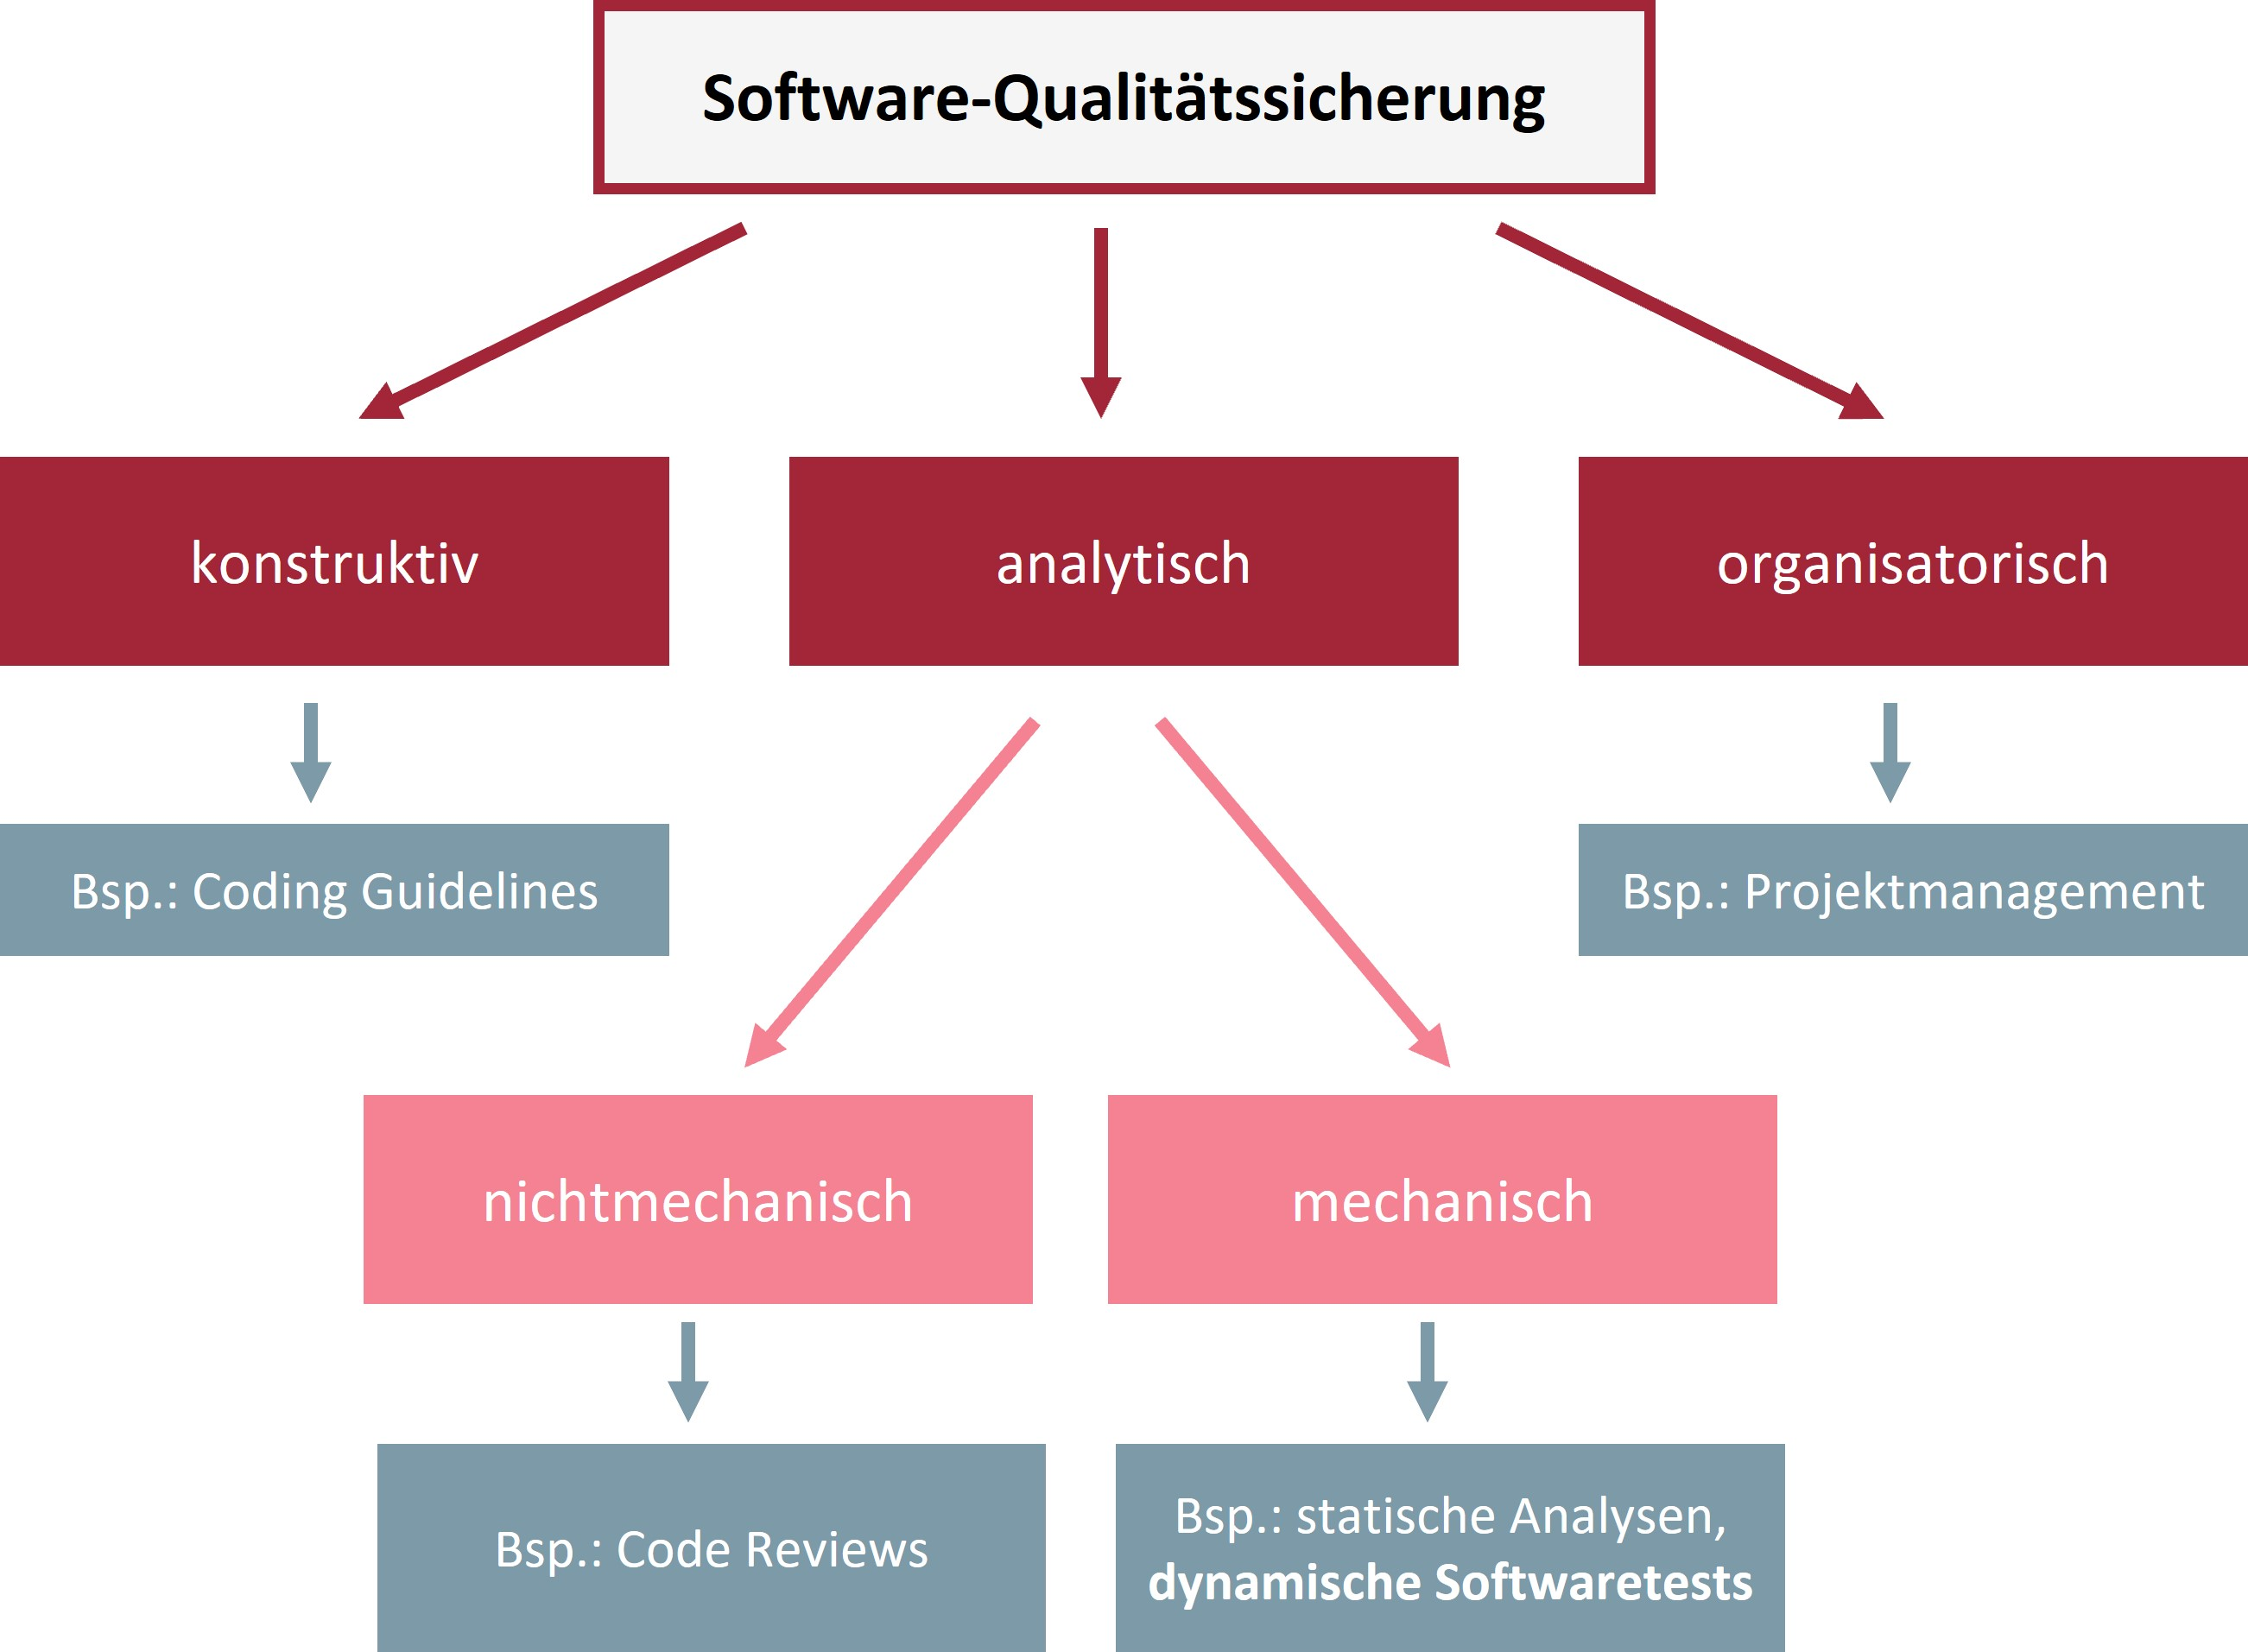
\includegraphics[width=0.5\columnwidth]{images/Qualitaetssicherung_Uebersicht.jpg}
\caption{Die verschiedenen Komponenten der Qualitätssicherung in der Software-Entwicklung in der Übersicht \cite[S. 271]{ludewig2010software}.}
\label{fig:qualitaetssicherung}
\end{figure}


Als Teilgebiet der Qualitätssicherung ist das dynamische Softwaretesten also ein wesentlicher Bestandteil bei der Sicherstellung der Produktqualität, deren wichtigsten Anforderungskriterien der ISO-/IEC-Standard 25010 \cite{ISO25010} als internationale Norm für Software und IT-Systeme zusammenfasst: Im Kern werden dabei von Softwareprojekten eine hohe Funktionalität, Effizienz, Sicherheit, Kompatibilität, Verlässlichkeit, Usability, Wartbarkeit und Portierbarkeit gefordert.

Dynamische Softwaretests besitzen demnach im übergeordneten Sinne die Aufgabe, diese Anforderungen zu prüfen und sicherzustellen. Im Konkreten bedeutet dies, dass dynamische Softwaretests anhand vordefinierter Testfälle mögliche Fehler vor der tatsächlichen Nutzung der Software aufdecken sollen und zudem überprüfen, ob ein Softwaresystem die an das System gestellten Spezifikationen erfüllt \cite[S. 246]{sommerville2012software-engineering}. Testfälle werden typischerweise entweder anhand eines systematischen Vorgehens künstlich erstellt oder ergeben sich aus Erfahrungswerten beziehungsweise der laufenden Produktion (vgl. dazu \autoref{subsec:beispieleTests}).  

Der Begriff des Fehlers kann dabei im Rahmen des Testens von Software vielschichtig interpretiert werden und nimmt unterschiedliche Rollen ein: Ein Fehlverhalten (engl.: failure) bezieht sich auf ein unerwartetes Ergebnis eines Programms, ein Codefehler (engl.: defect) beschreibt die zugehörigen fehlerhaften Codezeilen und ein Denkfehler (engl.: error) ist ein konzeptioneller Fehler, welcher vor der tatsächlichen Implementierung erfolgt. Alle drei Fehlerdefinitionen sind eng miteinander verknüpft: Ein Denkfehler kann bereits in der Konzeption dazu führen, dass trotz einer mutmaßlich korrekten Implementierung Codefehler und somit unterschiedliches Fehlverhalten auftreten können. Gleichzeitig kann es auch bei der Implementierung durch menschliches Versagen zu Codefehlern kommen, die in der Konzeption korrekt waren und somit keinen Denkfehler darstellen. Abbildung \ref{fig:fehler} zeigt die logische Struktur dieser Begrifflichkeiten auf und greift diese Thematik auf.

\begin{figure}[!h]
\centering
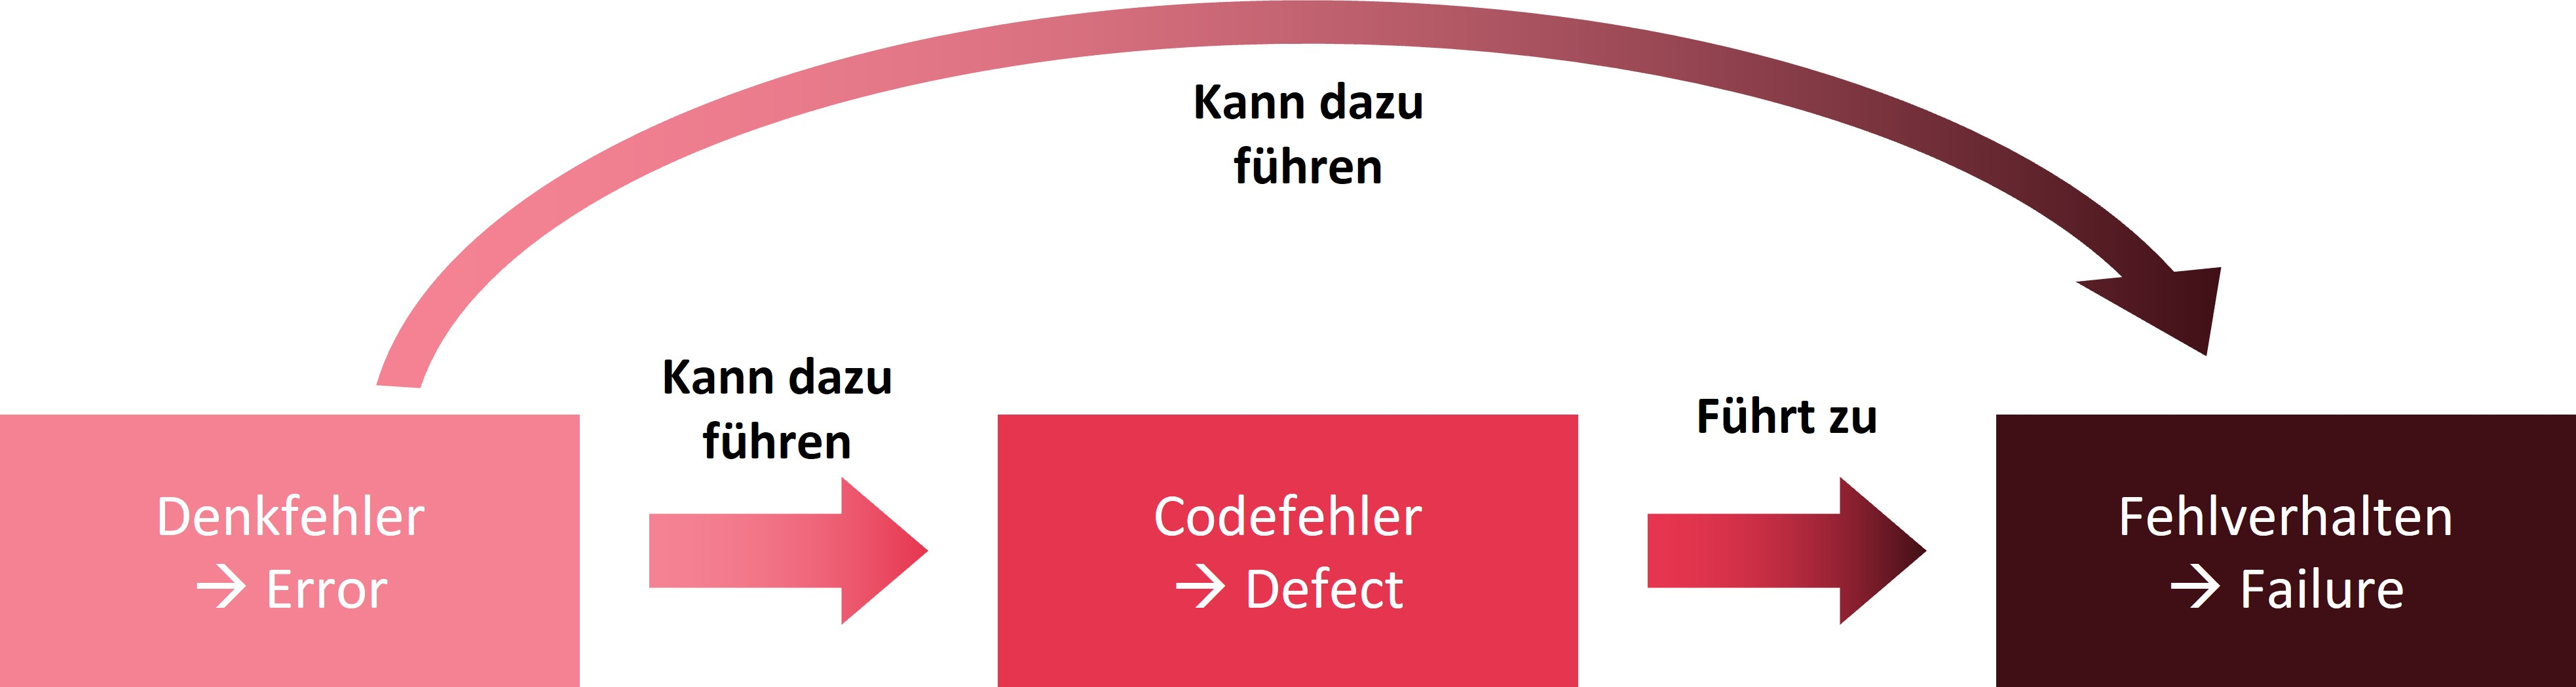
\includegraphics[width=0.8\columnwidth]{images/Fehler_Definition.jpg}
\caption{Ein Denkfehler bei der Implementierung führt zu einem Codefehler, welcher wiederum ein Fehlverhalten der Software auslöst.}
\label{fig:fehler}
\end{figure}

Grundsätzlich gilt es zu berücksichtigen, dass dynamische Softwaretests nicht in der Lage sind, alle Fehler eines Systems vollumfänglich aufzudecken \cite[S. 247]{sommerville2012software-engineering}. Dafür sind die zu testenden Systeme meist zu komplex und vollumfängliche Tests, wie in \autoref{subsec:abdeckung} aufgeführt, nicht umsetzbar. Software-Engineering Pionier Edward Dijkstra stellte in diesem Zusammenhang bereits 1972 fest: \glqq Tests können nur die Anwesenheit von Fehlern aufzeigen, nicht ihre Abwesenheit\grqq{} \cite{dahl1972structured}.

Spillner et al. \cite[S. 8]{spillner2011software} fassen die Kernaufgaben, welche dynamische Softwaretests erfüllen sollen, unter folgenden Aspekten zusammen:
\begin{itemize}
\item Entdeckung von Fehlverhalten innerhalb der betroffenen Software
\item Schaffung von Vertrauen in das System bei allen betroffenen Stakeholdern
\item Anregung frühzeitiger Analyse und Dokumentation in der Entwicklung und Wartung um Codefehler zu verhindern
%\item Messung von Software-Qualität durch Metriken wie zum Beispiel die Anzahl an Codezeilen, die zyklomatische Komplexität von McCabe \cite{mccabe1976complexity} oder Halsteads-Softwaremetriken \cite{halstead1977elements}%
\end{itemize}

\subsection{Testfall-Design}\label{subsec:testfallDesign}

Dynamische Softwaretests werden durch mehrere konkrete Tests an einem bestimmten Testsystem durchgeführt. Jeder Test unterliegt dabei einem spezifischen Testfall, der alle erforderlichen Komponenten zur Durchführung eines Tests bereithält. Diese sind die komplette Systemumgebung, Eingabedaten und das erwartete Verhalten beziehungsweise die erwartete Ausgabe des Systems \cite[S. 86]{schneider2012abenteuer}. 

Ein Testfall sollte dabei auf sinnvolle Art und Weise entwickelt werden: Dazu gehört laut Ludewig und Lichter \cite[S. 480]{ludewig2010software} eine eindeutig definierte Systemumgebung, ein systematisches Vorgehen bei der Wahl der Eingabedaten, klare Kriterien zur Testevaluation und eine detaillierte Dokumentation der Testergebnisse. Wenn diese vier Aspekte auf einen Testfall zutreffen, sprechen Ludewig und Lichter von einem \glqq systematischen Test\grqq{}.

Eine der wesentlichen Herausforderungen des dynamischen Softwaretestens besteht darin, ein derartiges systematisches Vorgehen zu entwickeln, um Testfälle möglichst effizient zu erzeugen: Grundsätzlich ist das Ziel des Testfall-Designs, mit möglichst wenig Aufwand, also einer geringen Anzahl an Testfällen, möglichst viele Fehler im Sinne eines Fehlverhaltens zu entdecken \cite[S. 498]{ludewig2010software}. Dabei sollte laut Ludewig und Lichter \cite[S. 498]{ludewig2010software} ein Testfall möglichst repräsentativ für viele andere Testfälle und zudem idealerweise sehr fehlersensitiv und redundanzarm sein.

Um diese Anforderungen abdecken zu können, wurden in der Vergangenheit verschiedene Techniken ausgearbeitet, die ein systematisches und effizientes Testfall-Design vereinfachen sollen. Dabei entstanden verschiedene Grundprinzipien, die sich aus einer unterschiedlichen Betrachtungsweise auf ein Softwaresystem ergeben. Diese sind nicht komplementär zu verstehen, sondern vielmehr ergänzend zur genauen Spezifizierung der Testfälle. Im Folgenden werden drei relevante Betrachtungsweisen vorgestellt: Stufenbasiertes Testen, Black Box- \& White-Box-Tests und Abdeckungsbasiertes Testen.

Konkrete Testmethoden wie beispielsweise Combinatorial Testing (vgl. \autoref{sec:combinatorialTesting}) oder die Äquivalenzklassenmethode (vgl. \autoref{subsec:beispieleTests}) lassen sich demnach meist unterschiedlichen Bereichen der aufgeführten Betrachtungsweisen zuordnen: So ist die Äquivalenzklassenmethode genauso wie das Combinatorial Testing auf fast allen Stufen des stufenbasierten Testens anwendbar, aber zugleich dem Black-Box-Ansatz zuzuordnen. Im Bereich des abdeckungsbasierten Testens spielt die Äquivalenzklassenmethode zudem bei der Abdeckung der Eingabewerte eine wichtige Rolle.

\subsubsection{Stufenbasiertes Testen}\label{subsec:stufen}

Das stufenbasierte Testen ist eine der abstraktesten Betrachtungsweisen im Hinblick auf die Erstellung von Testfällen: Basierend auf verschiedenen Stufen innerhalb eines Softwareprojekts werden beim stufenbasierten Testen Testfälle passend zu den Anforderungen und Aktivitäten im jeweiligen Stadium des Projekts erarbeitet \cite[S. 5]{ammann2008introduction}. 

Dabei kann auf verschiedene Stufen klassischer Prozessmodelle in der Softwareentwicklung zurückgegriffen werden: Häufig dient dabei das V-Modell als Basis, das im Auftrag des Bundesministeriums für Verteidigung entwickelt wurde und in der Softwarewelt in angepasster Form verbreitete Anerkennung fand \cite[S. 190]{ludewig2010software}. Das V-Modell ist als eine Weiterentwicklung des von Royce \cite{royce1987managing} 1970 entwickelten Wasserfallmodells zu verstehen: Dieses sieht vor, dass die Entwicklung eines Produkts im Allgemeinen in verschiedene Phasen unterteilt wird, bei der jede vorhergehende Phase essenzielle Grundlage der folgenden Phase ist \cite[S. 57 f.]{sommerville2012software-engineering}. Das V-Modell erweitert diesen Ansatz, indem aus jeder dieser Phasen des V-Modells Testfälle passend zu den jeweiligen Aktivitäten dieser Phase abgeleitet werden \cite[S. 190]{ludewig2010software}. %Bei der Anwendung von Test-Driven-Development \cite{beck2003test} werden die Testfälle dabei zusätzlich vor der eigentlichen Formulierung der Spezifikation beziehungsweise Implementierung vorgenommen. 

Üblicherweise werden dabei die folgenden Phasen aus dem Wasserfall- und V-Modell übernommen und daraus resultierende Testfälle unterschieden \cite[S. 5 f.]{ammann2008introduction}. Abbildung \ref{fig:vmodell} visualisiert die hierarchische Struktur und das Zusammenspiel der verschiedenen Stufen des V-Modells:
\begin{itemize}
\item Anforderungsanalyse \& Abnahmetests: Zu Beginn eines jeden Softwareprojekts  werden die konkreten Anforderungen in Zusammenarbeit mit dem Auftraggeber herausgearbeitet. Diese Anforderungen werden in einem abschließenden Stadium eines Projekts anhand von Abnahmetests mittels echter Daten von tatsächlichen oder potenziellen Nutzern getestet.
\item Systemarchitektur \& Systemtest: Beim Systementwurf werden konkrete Designentscheidungen bezüglich der grundlegenden Architektur von Software beschlossen, insbesondere die Zuordnung bestimmter Anforderungen an unterschiedliche Hard- und Softwarekomponenten. Aus dieser Phase resultieren Systemtests, die sämtliche Komponenten des Projekts auf Basis der Architektur testen. 
\item Systementwurf \& Integrationstest: Während der Systementwurf sich auf die grundlegende Architektur fokussiert, werden in der Phase des Subsystementwurfs die konkreten Strukturen und Komponenten der zu entwickelnden Software spezifiziert. Um die Interoperabilität dieser verschiedenen Komponenten zu testen, werden Integrationstests formuliert.
\item Software-Design/Implementierung \& Modul-/Unit-Tests: Die Implementierung umfasst die konkrete Umsetzung des Softwareentwurfs in Programmcode. Jede der einzelnen Komponenten, die meist unabhängig voneinander entwickelt werden, können mittels Unit-Tests bezogen auf kleine Einheiten wie Packages, Methoden oder Klassen getestet werden. Je nach Komplexität des Softwaresystems können weitere übergeordnete Module oberhalb der kleinsten Einheiten ausgearbeitet werden. Bevor letztlich mehrere Komponenten gemeinsam getestet werden, können einzelne Module vorgeschaltet in Modultests geprüft werden.
\end{itemize}

\begin{figure}[!htb]
\centering
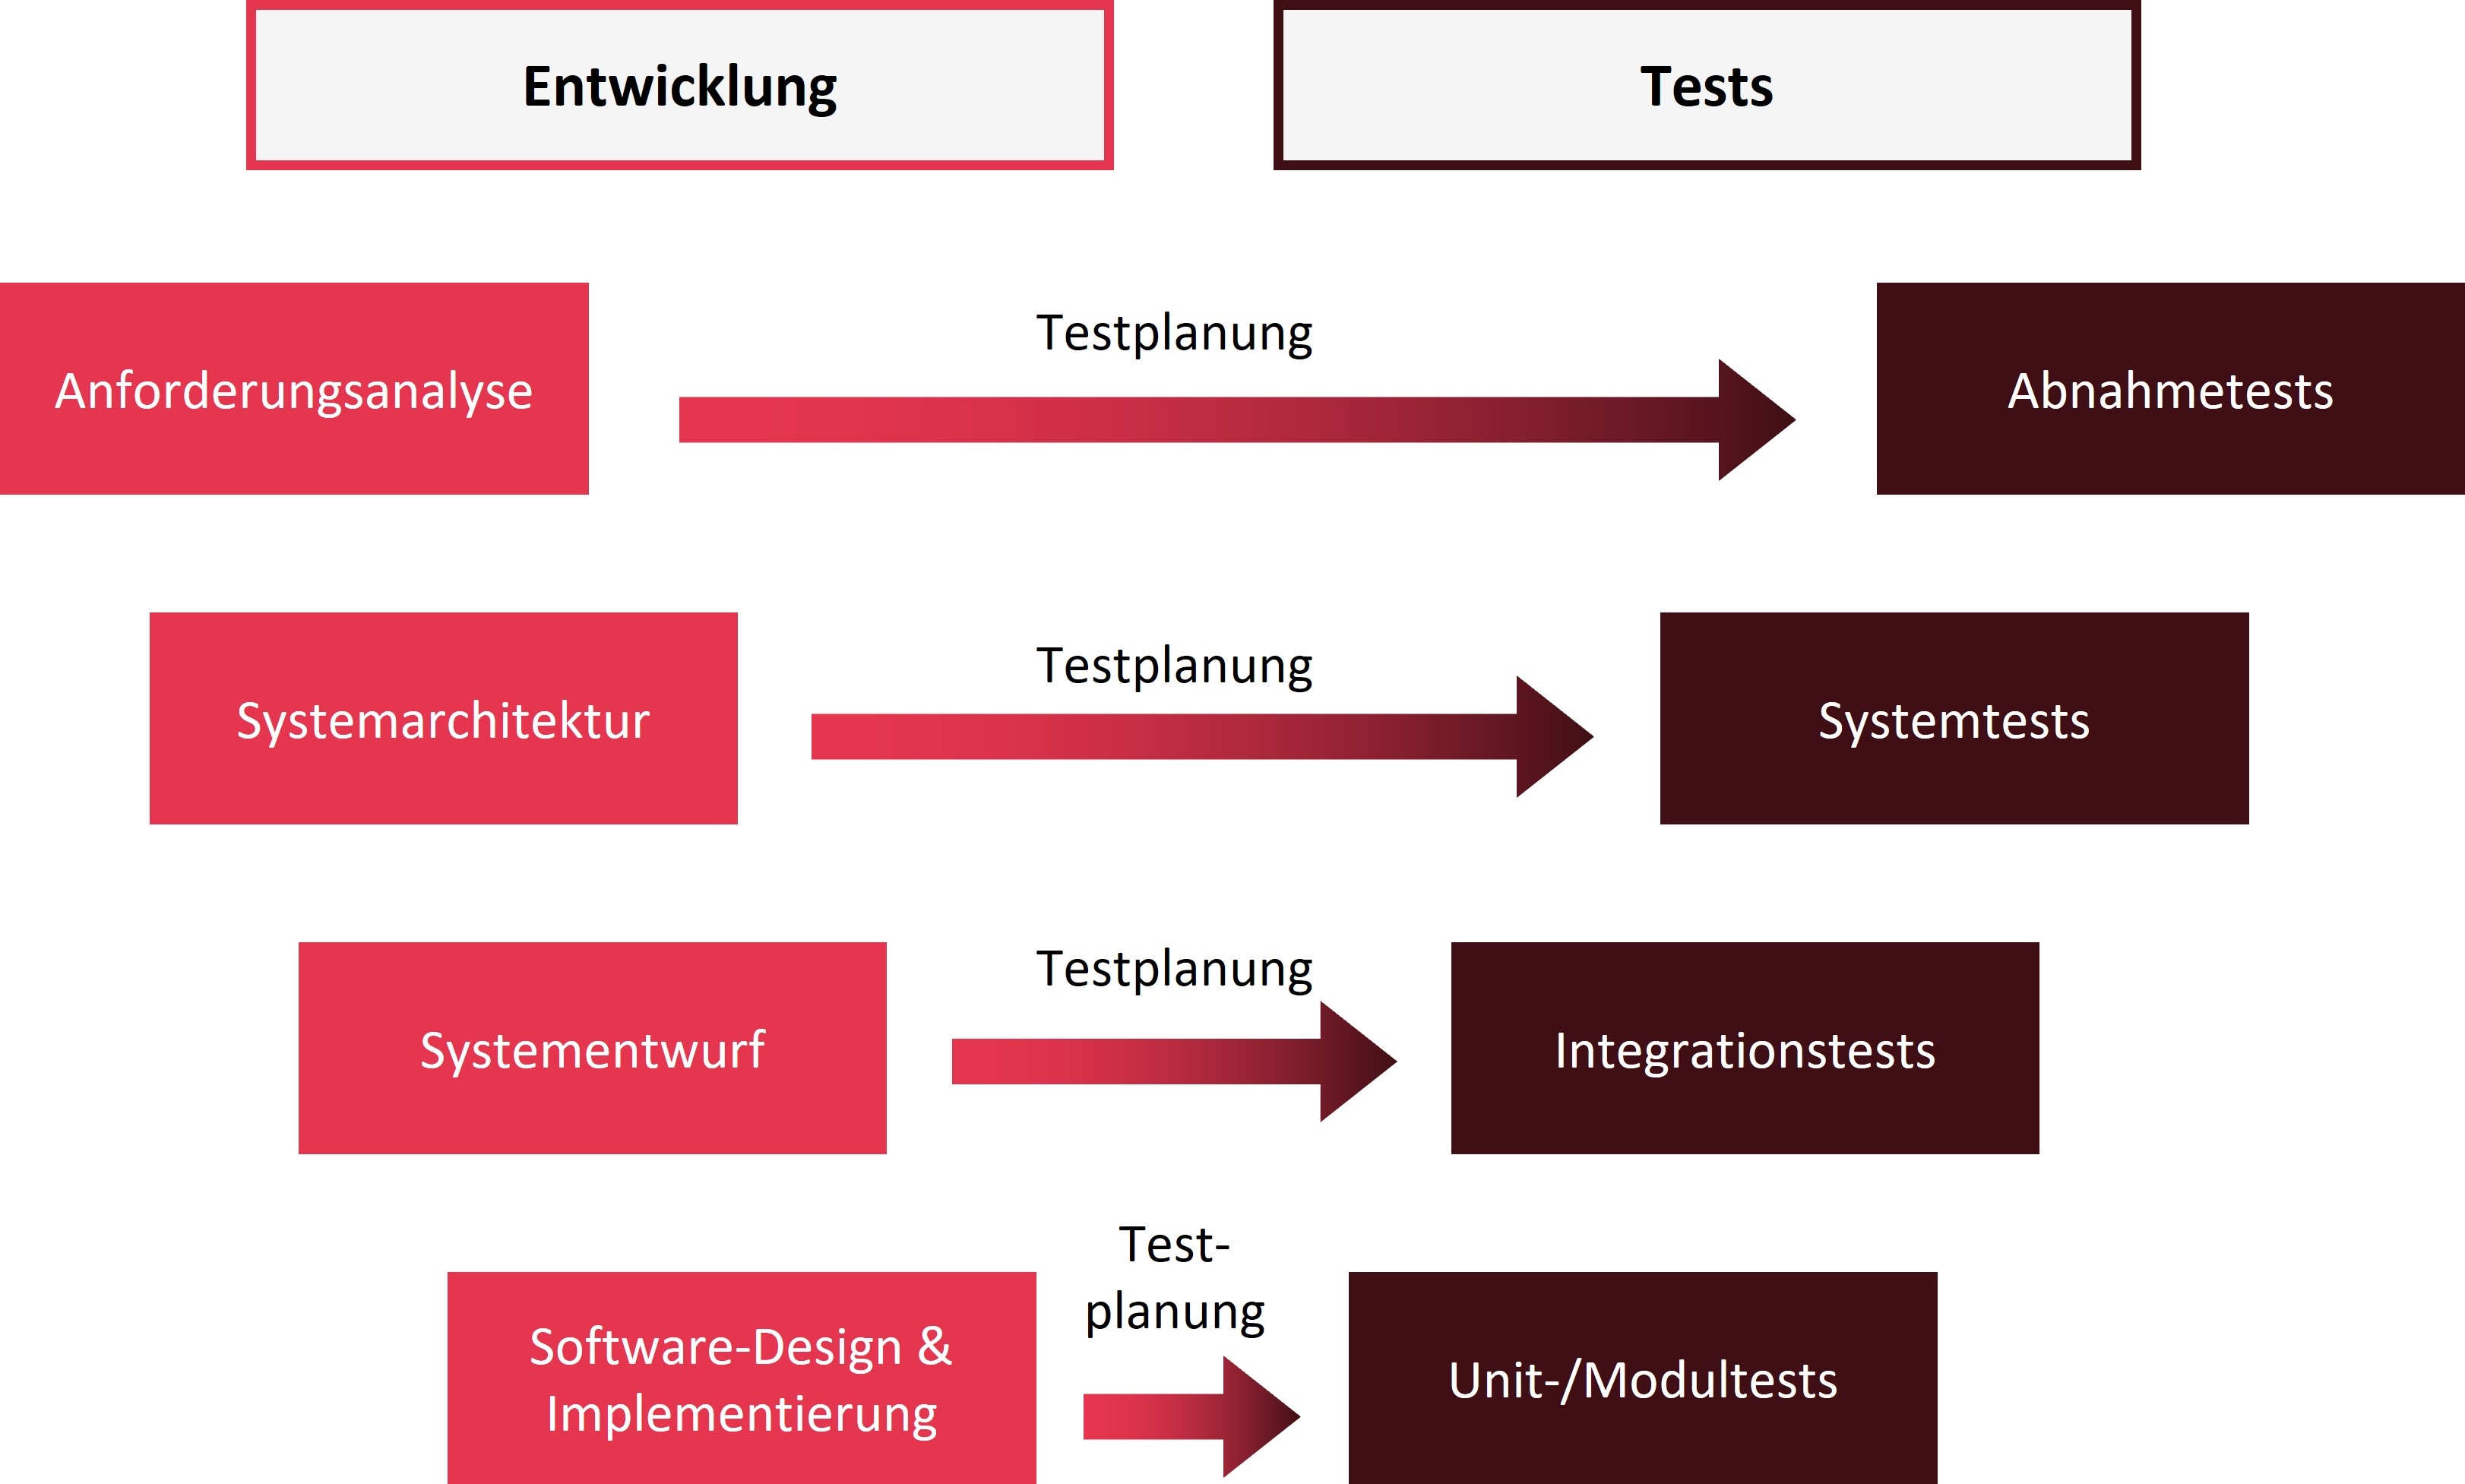
\includegraphics[width=0.7\columnwidth]{images/V_Modell.jpg}
\caption{Das V-Modell dient als Grundlage für das stufenbasierte Testen. Verschiedene Phasen im Entwicklungsprozess einer Software werden mit unmittelbaren Testfällen verknüpft \cite[S. 101]{craig2002systematic}.}
\label{fig:vmodell}
\end{figure}


Die Umsetzung des stufenbasierten Testens muss jedoch nicht unbedingt anhand der vorgegebenen Stufen des V-Modells erfolgen, sondern erlaubt auch selbstdefinierte Phasenmodelle: Craig und Jaskiel \cite[S. 98 f.]{craig2002systematic} führen beispielsweise bestimmte Produktrisiken, personelle oder zeitliche Anforderungen als wesentliche Faktoren bei der Stufenbildung auf.

%Unabhängig von der Wahl der Stufen erfordert das stufenbasierte Testen laut Craig und Jaskiel \cite[S. 98]{craig2002systematic} eine klare Struktur und Definition der Teststufen: Als wesentliche Komponenten müssen demnach die betroffenen Stakeholder und deren Interessen, die Hardware, die Software, die Schnittstellen und die notwendigen Daten im Vorfeld genau bestimmt werden.

\subsubsection{White Box- \& Black Box-Tests}\label{subsec:blackboxWhitebox}

Neben der Fokussierung auf die verschiedenen Phasen im Softwareentwicklungsprozess orientiert sich die Literatur bei der Erstellung von Testfällen in den meisten Fällen an der Unterscheidung zwischen Black-Box- und White-Box-Tests. Dabei bezieht sich der Begriff White-Box beziehungsweise Black-Box darauf, inwiefern die Struktur der zu testenden Softwareeinheit bei der Erstellung der Testfälle bekannt ist.

\paragraph{Black Box-Tests}

Beim Black-Box-Testen ist die Struktur der zu testenden Softwareeinheit wie beispielsweise der Aufbau des Programmcodes unbekannt, einzig und allein Beschreibungen der Software-Spezifikationen dienen als Grundlage für den Testfall \cite[S. 91]{schneider2012abenteuer}. Die Spezifikationen können dabei je nach Entwicklungsstadium im Stufenmodell (vgl. \autoref{subsec:stufen}) unterschiedlich aussehen und somit zu verschiedenen Testfällen führen: So basieren Abnahmetests im Wesentlichen auf dem Black-Box-Ansatz, werden aber auf eine gänzlich andere Art und Weise durchgeführt als Unit-Tests, die ebenfalls im Rahmen eines Black-Box-Ansatzes umgesetzt werden können.

Laut Schneider \cite[S. 91]{schneider2012abenteuer} sollen im Rahmen von Black-Box-Tests alle definierten Anforderungen an ein System getestet werden: Meist liegen diese nur in Form von Fließtext oder Tabellen vor und müssen dementsprechend in sinnvolle Testfälle umgewandelt werden \cite[S. 92]{schneider2012abenteuer}. Im Falle der Stufe der Anforderungsanalyse und Abnahmetests sind diese schriftlichen Beschreibungen beispielsweise textuelle Erläuterungen der Softwarefunktionalität, bei der Implementierung und Unit-Tests können dies unter anderem Methodenkommentare sein.

Verschiedene Methoden wie beispielsweise die Äquivalenzklassenmethode, die Grenzwertanalyse oder das zustandsbasierte Testen können den Black-Box-Tests zugeordnet werden(vgl. \cite[S. 94 ff.]{schneider2012abenteuer}). Details hierzu folgen in \autoref{subsec:beispieleTests}.

\paragraph{White Box-Tests}

Im Gegensatz zu den Black-Box-Tests setzen White-Box-Tests, oder auch Glass-Box-Tests genannt, voraus, dass die zu testende Softwareeinheit durchsichtig in ihrer Struktur ist und somit Testfälle auf Basis dessen erstellt werden können \cite[S. 91]{schneider2012abenteuer}. Konkret möchte man laut Schneider \cite[S. 91]{schneider2012abenteuer} bei White-Box-Tests kritische Stellen im Programmcode oder an den Schnittstellen verschiedener Softwarekomponenten anhand einer Analyse der vorhandenen Softwarestruktur entdecken.

Die meiste Verwendung finden White-Box-Test auf der Modul- und Implementierungsebene. Dort entsteht laut Schneider durch den hohen Grad an individueller Entwicklungsarbeit oftmals eine hohe Komplexität im Softwaresystem, welche zu schwer ermittelbaren Fehlverhalten im Code führen kann \cite[S. 108]{schneider2012abenteuer}. Daher soll laut Schneider \cite[S. 108 ff.]{schneider2012abenteuer} mit White-Box-Tests im Wesentlichen sichergestellt werden, dass alle geschriebenen Programmteile auch tatsächlich verwendet werden. Dies wird meist mittels Maßen für die Codeüberdeckung umgesetzt: Metriken der Anweisungsüberdeckung, Zweigüberdeckung und Pfadüberdeckung werden dafür in vielen Fällen als Gütemaß herangezogen \cite[S. 109 ff.]{schneider2012abenteuer}. 

Die Messbarkeit der Güte eines Testverfahrens steht zunehmend nicht nur bei den Methoden des White-Box-Testens im Vordergrund wie der folgende Unterunterabschnitt zum abdeckungsbasierten Testen aufzeigt: Die Messung der Anweisungsüberdeckung, Zweigüberdeckung und Pfadüberdeckung stellt dabei einen relevanten Vertreter der Abdeckungsprüfung von Testverfahren im Kontext von Graphen-basierter Abdeckung dar.

\subsubsection{Abdeckungsbasiertes Testen}\label{subsec:abdeckung}

Während sich die Literatur in der Vergangenheit bei der Testfallentwicklung im Wesentlichen auf die zuvor aufgeführten Perspektiven der Phasen auf Prozessebene (vgl. \autoref{subsec:stufen}) und der Sichtbarkeit der Struktur von Software (vgl. \autoref{subsec:blackboxWhitebox}) fokussierte, rückt zunehmend eine weitere dritte Betrachtungsweise in den Fokus der Forschung: Auf Basis von verschiedenen Metriken, welche Abdeckungen bestimmter Eigenschaften des Softwaresystems messen, steht beim abdeckungsbasierten Testen vor allem die Quantifizierung der Güte eines Testverfahrens zur Sicherstellung der Softwarequalität im Fokus \cite{craig2002systematic}. Diese quantitativen Verfahren können unter anderem helfen, verschiedene Stakeholder eines Softwareprojekts von der Güte eines Testbestandes zu überzeugen \cite{kuhn2010practical}.

Neben dem Ansatz, durch verlässliche Metriken Vertrauen in eine Menge von Testfällen zu schaffen, basiert das Konzept des abdeckungsbasierten Testens auf der Erkenntnis, dass ein vollständiges Testen aller denkbaren Zustände, die ein Softwaresystem einnehmen kann, unmöglich ist \cite[S. 16 f.]{ammann2008introduction}. Konkret führen Ammann und Offutt \cite[S. 16]{ammann2008introduction} das Beispiel eines Java Compilers an, dessen Limitierung durch die maximale Kapazität des Compiler-Parsers gegeben ist. Der Java Compiler kann theoretisch jede beliebige Zeichenfolge einer .java-Datei aufnehmen, versucht diese anhand seiner internen Logik zu interpretieren und daraus ein ausführbares Programm in Maschinencode zu erzeugen. Die Länge der Eingabe ist durch die Menge an Zeichen limitiert, die der zugehörige Parser aufnehmen kann: Dies entspricht im Falle von Java bei einer maximalen Dateimenge von 64 kB pro Methode \cite{deva_2021} und einer UTF-8-Kodierung mit 1 bis 4 Bytes pro Zeichen mindestens einer Anzahl von 16.000 Zeichen bei voller Auslastung der 64 kB. Berücksichtigt man nun noch alle denkbaren Kombinationen, die durch Permutieren der 144.697 aktuell im Unicode belegten Zeichen \cite{unicode} zustande kommen können, so ergibt sich eine Mindestanzahl von $16.000^{144.697}$ verschiedenen Kombinationen, die ein Java-Parser berücksichtigen müsste: Eine Dimension, die kein Rechner auf dieser Welt testen kann.

Dementsprechend können Testfälle meist nur einen Anteil aller denkbaren Kombinationen abdecken, sodass es sehr hilfreich ist, die Qualität einer Menge an Testfällen beurteilen zu können: Dies wird beim abdeckungsbasierten Testen durch die Nutzung von quantifizierbaren Metriken vorgenommen \cite[S. 17]{ammann2008introduction}. Jeder Testfall kann bei seiner Durchführung ein Testkriterium erfüllen oder auch nicht, sodass sich über die gesamte Menge aller zusammenhängender Testfälle ein Anteil ergibt, der die Erfüllung des Testkriteriums im Gesamten quantifiziert \cite[S. 17]{ammann2008introduction}. 

Konkret bedeutet dies: Für jedes Abdeckungskriterium lässt sich bestimmen, welche Eigenschaften die Menge aller Testfälle benötigt, um das Kriterium vollständig zu erfüllen. Bei Combinatorial Testing sind dies beispielsweise alle $t$-fachen Kombinationsabdeckungen (vgl. \autoref{subsec:abdeckung}) der Eingabevariablen. Die Quantifizierung der Güte der Menge aller Testfälle ergibt sich schließlich durch die Quote der erfüllten Eigenschaften, die das Abdeckungskriterium fordert. Jeder Testfall kann dann seinen Teil dazu beitragen, dass das betroffene Kriterium erfüllt wird. Dabei kann es passieren, dass mehrere Testfälle den \glqq gleichen\grqq{} Beitrag im Sinne des Testkriteriums liefern. In anderen Worten: Manche Testfälle sind überflüssig, da die geforderte Eigenschaft des Abdeckungskriteriums bereits durch einen anderen Testfall oder die Kombination mehrerer Testfälle abgedeckt wird. 

%Grundsätzlich gelten auch beim abdeckungsbasierten Testfalldesign die Prinzipien eines guten Testfalldesigns mit einer hohen Fehlererkennungsrate bei möglichst geringem Testaufwand \cite[S. 20 f.]{craig2002systematic}. Zudem lassen sich manche Abdeckungskriterien insofern vergleichen, als sich diese gegenseitig ergänzen: Beispielsweise ist im Falle der Codeüberdeckung (vgl. \autoref{subsec:beispieleTests}) die Zweigüberdeckung als eine Erweiterung der Anweisungsüberdeckung zu verstehen.

Ammann und Offutt \cite{ammann2008introduction} unterscheiden vier wesentliche Kategorien von Abdeckungen im Bereich des dynamischen Softwaretestens. 
\begin{itemize}
\item Graphen-basierte Abdeckung orientiert sich an verschiedenen Graphstrukturen, die sich im Rahmen eines Softwarekonzepts ergeben wie beispielsweise die Verzweigungen und Wiederholungen innerhalb des Programmcodes. Dabei können Metriken wie Knoten- oder Kantenabdeckungen zur Quantifizierung der Abdeckung herangezogen werden \cite[S. 27 ff.]{ammann2008introduction}.
\item Logische Abdeckung basiert auf den Prinzipien der Prädikatenlogik, die sich analog zu Graphstrukturen auf verschiedene Bereiche eines Softwaresystems anwenden lassen, unter anderem die Verzweigungen innerhalb des Programmcodes oder die Umformulierung von Anforderungsspezifikation in Wenn-dann-Verbindungen \cite[S. 131 ff.]{ammann2008introduction}. Die Abdeckung der daraus abgeleiteten Testfälle kann mit Methoden der Prädikatenlogik wie beispielsweise der Klausel- und Prädikatenabdeckung gemessen werden \cite[S. 106 ff.]{ammann2008introduction}.
\item Die Abdeckung der möglichen Eingabewerte berücksichtigt die Grundvoraussetzung jedes Softwaresystems: Jedes Programm verwendet in gewisser Weise Eingaben, sodass alle beliebigen Softwaretests auch Elemente des Eingabeuniversums verwenden \cite[S. 150]{ammann2008introduction}. Insbesondere dann, wenn die Struktur einer Software unbekannt ist, stellt die Analyse der möglichen Eingaben und Ausgaben gemeinsam mit der Anwendung von Erfahrungswerten die einzige Möglichkeit zum Testen von Softwareeinheiten dar. Im Vergleich zu den anderen abdeckungsbasierten Ansätzen stehen beim expliziten Testen der Eingabewerte die kombinatorischen Eingabemöglichkeiten im Vordergrund \cite[S. 150 ff.]{ammann2008introduction}. Combinatorial Testing ist dabei die relevanteste Methode zur Umsetzung dieser Strategie, welche im Folgenden in \autoref{sec:combinatorialTesting} ausführlich vorgestellt wird. 
\item Syntax-basierte Abdeckung verwendet die Ideen der Automatentheorie und benutzt dabei syntaktische Beschreibungen von zu testenden Softwareeinheiten, um Testfälle abzuleiten \cite[S. 170 ff.]{ammann2008introduction}. Im Zusammenhang mit Programmcode spielt vor allem der Begriff der Mutationen eine wichtige Rolle, bei dem elementare Codestücke durch leichte Veränderungen ersetzt werden und so Fehlverhalten provoziert wird. Als Metrik werden dabei zumeist die Abdeckung der Symbole und Produktionsregeln und weitere komplexere Kombinationen verwendet \cite[S. 172]{ammann2008introduction}.
\end{itemize}


\begin{comment}
Ammann und Offutt \cite{ammann2008introduction} unterscheiden vier wesentliche Kategorien von Abdeckungen im Bereich des Softwaretestens. 
\begin{itemize}
\item Graphen-basierte Abdeckung: Typischerweise verbindet man Graphen in den ersten Phasen des Softwareentwicklungsprozesses der Anforderungsanalyse und der Systemarchitektur mit Anwendungsfalldiagrammen oder Aktivitätsdiagrammen. Weitere Graphstrukturen lassen sich zudem auf der Modul- und Implementierungsebene bei Komponenten- und Klassendiagrammen finden. Im Zusammenhang mit der Generierung von Testfällen sind jedoch vor allem Zustandsmaschinen und insbesondere Anweisungsabläufe und Datenflüsse weit verbreitet. All diese Graphenmodelle können laut Ammann und Offutt \cite[S. 27 ff.]{ammann2008introduction} auf Basis verschiedener Graphen-basierter Metriken getestet werden. Dabei unterscheiden die beiden Autoren zwischen Abdeckungskriterien der strukturellen Eigenschaften und des Datenflusses der zu testenden Softwareeinheit. Beide Varianten fokussieren sich auf verschiedene Metriken der Knoten- und Kantenabdeckung beziehungsweise komplexeren Messzahlen der erzeugten Graphstruktur \cite[S. 33 ff.]{ammann2008introduction}.
\item Logische Abdeckung: In recht ähnlicher Art und Weise wie bei der Graphen-basierten Abdeckung orientieren sich die Testprinzipien der logischen Abdeckung in den meisten Anwendungsfällen an den Verzweigungen innerhalb des Programmcodes. Wenn-dann-Beziehungen und Wiederholungen können dabei in prädikatenlogische Aussagen umgewandelt werden, die schließlich als Grundlage für die Erzeugung von Testfällen dienen \cite[S. 120 ff.]{ammann2008introduction}. Neben diesem strukturbasierten Ansatz (analog zu einer White-Box-Strategie) lässt sich das Prinzip der Prädikatenlogik auf die Ebene der Spezifikation von verschiedenen zu testenden Softwareeinheiten übertragen, indem Vorbedingungen an den Testprüfling in prädikatenlogische Aussagen formuliert werden \cite[S. 131 ff.]{ammann2008introduction}. Zudem führen Ammann und Offutt die Möglichkeit auf, die Abläufe einer Zustandsmaschine in prädikatenlogische Aussagen umzuformulieren und diese zu testen \cite[S. 134 ff.]{ammann2008introduction}. Als Metrik werden bei der logischen Abdeckung in verschiedenen Ausprägungen die logisch denkbaren Möglichkeiten mit den tatsächlich getesteten Möglichkeiten abgeglichen (Klausel- und Prädikatenabdeckung) \cite[S. 106 ff.]{ammann2008introduction}.
\item Abdeckung der möglichen Eingabewerte: Eingaben und Ausgaben sind wesentliche Grundprinzipen einer jeden Software, sodass jede Art eines Softwaretests in gewisser Form Elemente des Eingabeuniversums verwendet \cite[S. 150]{ammann2008introduction}. Bei den zuvor aufgeführten Varianten der Graphen-basierten und logischen Abdeckung steht jedoch das Universum aller möglichen Eingaben selbst nicht im Mittelpunkt, sondern vielmehr die Struktur und die Zusammenhänge innerhalb der Software. Beim Testen der Eingabewerten ist dies der Fall: Im Konkreten werden dabei die Eingabedomäne einer Softwareeinheit in verschiedene Mengen unterteilt und anschließend anhand kombinatorischer Metriken die Qualität der resultierenden Softwaretests ermittelt \cite[S. 150 ff.]{ammann2008introduction}. Dabei kann laut Ammann und Offutt im Wesentlichen zwischen einer unabhängigen Betrachtungsweise auf einzelne Parameter, also beispielsweise die verschiedenen denkbaren Werte einer Variablen, und einer gesamtheitlichen Sichtweise auf die Funktionalität im Zusammenspiel verschiedener Parameter unterschieden werden \cite[S. 153 ff.]{ammann2008introduction}. Combinatorial Testing (vgl. \autoref{sec:combinatorialTesting}) ist dabei eine der relevantesten Methoden zur Umsetzung dieser Strategie.
\item Syntax-basierte Abdeckung: Die Grundidee des Syntax-basierte Testens stammt im Wesentlichen aus Bereichen der Automatentheorie und verwendet syntaktische Beschreibungen von zu testenden Softwareeinheiten um Testfälle abzuleiten \cite[S. 170 ff.]{ammann2008introduction}. So lässt sich beispielsweise ein Programmiersprache über eine BNF-Grammatik mit verschiedenen Symbolen und Produktionsregeln definieren, die als Grundlage für eventuelle Testfälle dienen. Als Metrik werden dabei die Abdeckung der Symbole und Produktionsregeln und weitere komplexere Kombinationen verwendet \cite[S. 172]{ammann2008introduction}. Im Zusammenhang mit Programmcode spielt jedoch vor allem der Begriff der Mutationen eine wichtige Rolle, bei dem elementare Codestücke durch leichte Veränderungen ersetzt werden. Als Beispiele führen Ammann und Offutt unter anderem das Austauschen von arithmetischen Operationen an \cite[S. 182 ff.]{ammann2008introduction}. Die Mutationen sollten in den meisten Fällen zu einem unerwünschten Verhalten der Software führen, sodass beispielsweise gemessen werden kann, wie häufig diese zu Fehlern führen \cite[S. 178 f.]{ammann2008introduction}.
\end{itemize}
\end{comment}



\subsection{Beispiele für Teststrategien}\label{subsec:beispieleTests}

Der folgende Abschnitt greift die grundlegende Herangehensweise in Bezug auf das dynamische Softwaretesten aus \autoref{subsec:testfallDesign} auf und führt einige konkrete Beispiele für Teststrategien ein. Diese Beispiele beschränken sich auf mögliche Anwendungen im Zusammenhang mit dem in \autoref{chap:anwendungsfall} vorgestellten Anwendungsfall. Da dieser sich im Wesentlichen auf einen spezifikationsbezogenen Ansatz fokussiert, werden insbesondere die Techniken des White-Box-Testens (vgl. \autoref{subsec:blackboxWhitebox}) an dieser Stelle ausgeklammert. Detaillierte Ausführungen zu den verbreiteten White-Box-Strategien der Anweisungs-, Zweig- und Pfadüberdeckung lassen sich in \cite[S. 108 ff.]{schneider2012abenteuer} nachlesen.

Da der Fokus dieser Arbeit auf Combinatorial Testing liegt, werden zudem die Prinzipien dieser Teststrategie nicht an dieser Stelle, sondern im folgenden, separaten \autoref{sec:combinatorialTesting} vorgestellt.

\subsubsection{Äquivalenzklassenmethode}\label{subsub:äquivalenklassenmethode}

Da vollständiges Testen - wie zuvor erläutert - nicht möglich ist, erfordern systematische Tests Einschränkungen bei der Wahl der Parameter. Die Äquivalenzklassenmethode löst dieses Problem derart, dass alle denkbaren Eingaben in verschiedene Äquivalenzklassen partitioniert werden \cite[S. 94]{schneider2012abenteuer}. Dabei sollten laut Schneider \cite[S. 94 ff.]{schneider2012abenteuer} die unterschiedlichen Klassen derart konstruiert werden, dass Vertreter aus derselben Klasse sich in Bezug auf das Fehlerverhalten innerhalb der Software identisch verhalten. Als Beispiel führt Schneider eine automatisierte Schwimmbadkasse auf, die für Jugendliche unter 18 Jahre einen vergünstigten Preis anbietet. In diesem Fall würde sich eine Äquivalenzklasse für die Variable \glqq Alter\grqq{} durch die Menge \glqq Jugendlich\grqq{} $= \{n < 18 ~ | ~ n \in \N\}$ und eine weitere Klasse \glqq Erwachsen\grqq{} $= \{n \geq 18 ~ | ~ n \in \N\}$ ergeben. 

Je nach Spezifikation und denkbaren Eingaben müssen die Äquivalenzklassen auch mögliche Falscheingaben berücksichtigen. Eine wesentliche Herausforderung bei Anwendung der Äquivalenzklassenmethode besteht laut Schneider darin, eine passende Auswahl der Klassen zu treffen, die einerseits nicht zu kleinteilig, andererseits aber auch nicht zu pauschalisierend sein sollte \cite[S. 95]{schneider2012abenteuer}.

\subsubsection{Grenzwertanalyse}\label{subsub:grenzwertanalyse}

Die Grenzwertanalyse basiert auf der Annahme, dass es häufig unmittelbar an den Grenzen verschiedener Eingabeparameter zu Fehlverhalten kommt, da diese oftmals nicht genau definiert sind oder von Programmierenden nicht berücksichtigt werden \cite[S. 120]{spillner2011software}. Dementsprechend überprüft die Grenzwertanalyse die Grenzen kritischer Werte und stellt somit eine Erweiterung der Äquivalenzklassenmethode dar \cite[S. 120 f.]{spillner2011software}. 

Für jede Äquivalenzklasse ergeben sich laut Spillner et al. \cite[S. 120 f.]{spillner2011software} automatisch kritische Grenzen, die mittels der Grenzwertanalyse abgedeckt werden können. Im Beispiel der Schwimmbadkasse würde dies bedeuteten, dass ein besonderes Augenmerk auf die Werte 17 und 18 gelegt werden sollte. Neben diesen offensichtlichen Grenzen der verschiedenen Äquivalenzklassen werden im Rahmen der Grenzwertanalyse häufig auch extreme, unerwartete Werte wie beispielsweise die maximal oder minimal mögliche Eingabe berücksichtigt \cite[S. 122]{spillner2011software}. Sowohl die Grenzwertanalyse als auch die Äquivalenzklassenmethode lassen sich auf allen Ebenen des Stufenmodells (vgl. \autoref{subsec:stufen}) anwenden und sind in Bezug auf das abdeckungsbasierte Testen vor allem im Bereich der Abdeckung der Eingaben relevant.

\begin{comment}
\subsubsection{Zustandsbasiertes Testen}

Zustandsbasiertes Testen basiert auf der grundlegenden Annahme, dass sich jeder deterministische Programmfluss einer Software durch einen endlichen Automaten mit verschiedenen Zuständen und exakt definierten Zustandsübergängen darstellen lässt. Die Darstellung eines endlichen Automaten kann über ein Graph-basiertes Modell (vgl. \autoref{subsec:abdeckung}) oder über eine Zustandsübergangstabelle erfolgen. Als Teststrategie eines Zustandsautomaten ergibt sich die Methode, dass jede einzelne Zelle der Zustandsübergangstabelle einen Testfall ergibt. Dadurch, dass die Transition der betroffenen Zustände im endlichen Automat eindeutig definiert sind, fällt die Ableitung der notwendigen Werte betroffener Parameter leicht. 

Das zustandsbasierte Testen spielt insbesondere dann eine wichtige Rolle, wenn Systeme verschachtelte Hierarchien besitzen. Im Anwendungsfall dieser Arbeit (vgl. \autoref{chap:anwendungsfall}) wird dies insbesondere bei Eingabemasken relevant, die nur durch die bestimmte Auswahl eines spezifischen Parameters zum Einsatz kommen und in allen anderen Fällen nicht. 

\end{comment}

\subsubsection{(Adaptive) Random Testing}\label{subsub:randomTesting}

In einigen Fällen möchte man eine Softwareeinheit testen, bei der weder eine detaillierte Beschreibung der Spezifikation noch der Programmcode selbst vorliegt. Dafür bietet sich die Verwendung des Zufallsprinzips an, welches die Grundlage des Random Testings ist. Dabei wird für das Eingabeuniversum eine Wahrscheinlichkeitsverteilung angenommen, aus welcher Eingabewerte zufällig entnommen werden \cite[S. 141 f.]{spillner2011software}. Grundsätzliche Vorteile einer zufallsbasierten Teststrategie ergeben sich laut Spillner \cite[S. 142]{spillner2011software} vor allem durch eine realitätsnahe Abbildung der tatsächlich verwendeten Werte der Softwareeinheit und durch die Möglichkeit, statistische Methoden zur Quantifizierung der Systemzuverlässigkeit anwenden zu können.

Unter anderem White und Cohen \cite{white1980domain} konnten herausfinden, dass Fehlverhalten meist sehr gebündelt in Bereichen von Eingabewerten auftreten, sodass bereits durchgeführte Testfälle, die kein Fehlverhalten aufdeckten, möglichst weit im Eingabeuniversum von neuen Testfällen entfernt sein sollten \cite{survey2013}. Aus diesem Grund entwickelten Chen et al. \cite{chen2004adaptive} die Methode des Adaptive Random Testing, welche versucht, die Testfälle möglichst weit und gleichmäßig über das Eingabeuniversum zu verteilen. Verschiedene Strategien und Algorithmen auf Basis von Distanzmaßen, Ausschlussverfahren oder evolutionären Algorithmen wurden in der Vergangenheit entwickelt, um Adaptive Random Testing in der Praxis umzusetzen \cite{huang2012adaptive}.

\subsubsection{Erfahrungsbasiertes Testen}\label{subsub:erfahrungsbasiertesTesten}

Neben den aufgeführten systematischen Ansätzen existiert eine weitere Methode zur Testfallerzeugung, die in der Anwendungspraxis eine bedeutende Rolle spielt: Erfahrungsbasiertes Testen kann vor allem Fehler aufdecken, die systematische Ansätze übersehen \cite[S. 210]{spillner2010basiswissen}. Das Wissen und die Expertise der testenden Person bildet dabei die Grundlage, um mögliche Probleme innerhalb einer Softwareeinheit mit Tests aufzudecken. Spillner et al. \cite[S. 213]{spillner2010basiswissen} betonen, dass erfahrungsbasiertes Testen nicht als erstes Mittel der Wahl bei der Erstellung von Testfällen verwendet werden sollte, sondern vielmehr als Ergänzung anderer systematischer Ansätze zu verstehen ist. 

Insbesondere interagiert das erfahrungsbasierte Testen häufig mit anderen konkreten Testmethoden wie beispielsweise der Äquivalenzklassenmethode oder der Grenzwertanalyse: So stellt die Wahl der Äquivalenzklassen beziehungsweise die Wahl kritischer Grenzwerte eine wesentliche Herausforderung der beiden Testmethoden dar, sodass an dieser Stelle Erfahrungswerte und Expertise besonders hilfreich sein können.

Erfahrungsbasiertes Testen lässt sich nur teilweise den drei zuvor aufgeführten Grundprinzipien des Testens zuordnen und kann selbst nur als \glqq semi-systematisches\grqq{} Verfahren bezeichnet werden: Die Methode lässt sich nicht eindeutig als Black Box- oder White Box-Technik einstufen \cite[S. 213]{spillner2010basiswissen}, auch ein Abdeckungskriterium, welches die Güte von erfahrungsbasierten Tests messen kann, existiert in den meisten Fällen nicht. Die Expertise erfahrenerer Tester*innen kann auf allen Ebenen des stufenbasierten Testens nützlich sein. Sie kommt jedoch meist auf höheren Teststufen zum Einsatz, da auf den niedrigeren Ebenen genügend Informationen über die Spezifikationen, wie beispielsweise der Programmcode selbst, zur Verfügung stehen \cite[S. 213]{spillner2010basiswissen}.

In der Praxis haben sich in Bezug auf erfahrungsbasiertes Testen verschiedene Teilaspekte herausgebildet \cite[S.210 ff.]{spillner2010basiswissen}:
\begin{itemize}
\item \glqq Error Guessing\grqq{} (deutsch: Fehlerraten) basiert auf der Idee, Fehler aus der Vergangenheit oder in Zukunft zu erwartende Fehler bei der Testfallerstellung zu berücksichtigen \cite[S.210 f.]{spillner2010basiswissen}.
\item Checklistenbasiertes Testen verwendet eine Checkliste zur Testfallerzeugung, die eine erfahrene Testperson in der Vergangenheit angelegt hat und die als Anleitung für zukünftige Testfälle dient \cite[S. 211 f.]{spillner2010basiswissen}. In diesem Fall kann ein Abdeckungskriterium für die Güte einer Menge von Testfällen definiert werden, indem der Anteil der erfüllten Aspekte der Checkliste ermittelt wird \cite[S. 211]{spillner2010basiswissen}.
\item Exploratives Testen ist ein Verfahren, das einen kontinuierlichen Prozess bestehend aus Testfallerzeugung und Auswertung jener Testfälle beschreibt \cite[S. 211]{spillner2010basiswissen}. Über die Zeit hinweg entwickelt laut Spillner und Linz \cite[S. 212]{spillner2010basiswissen} die testende Person zunehmend mehr Wissen und Verständnis über das Testobjekt und kann dieses für neue, verbesserte Testfälle anwenden. Darüber hinaus kann das Wissen des explorativen Testens angewendet werden, um systematische Tests zu entwickeln.
\end{itemize}

\section{Combinatorial Testing}\label{sec:combinatorialTesting}

Combinatorial Testing (deutsch: Kombinatorisches Testen) ist analog zu den Beispielen aus \autoref{subsec:beispieleTests} eine Strategie zur systematischen Erzeugung von Testfällen. Da diese Methode in dieser Arbeit im Mittelpunkt steht, wird diese an dieser Stelle ausführlicher als die zuvor aufgeführten Teststrategien vorgestellt. Zunächst sollen dabei die grundlegende Motivation für Combinatorial Testing und die wesentlichen Prinzipien im Fokus stehen. Anschließend werden verschiedene Metriken zur Quantifizierung der Güte eines Testbestandes im Zusammenhang von Combinatorial Testing erläutert und verschiedene Algorithmen und Tools zur Anwendung von Combinatorial Testing vorgestellt.

\subsection{Einführung in Combinatorial Testing}\label{subsec:einführungCombinatorial}

Als wesentliche Motivation für die Verwendung kombinatorischer Methoden bei der Erzeugung von Testfällen ergibt sich, wie bei fast allen Testfallstrategien, die Erkenntnis, dass vollständige Tests in der Realität nicht umsetzbar sind (vgl. \autoref{sec:einführungTest}). Combinatorial Testing greift diese Tatsache auf und versucht auf effiziente Art und Weise das Eingabeuniversum einer zu testenden Softwareeinheit möglichst sinnvoll mittels kombinatorischer Methoden im Sinne von quantifizierbaren Metriken (vgl. \autoref{subsec:abdeckung}) abzudecken. Dabei kann Combinatorial Testing auf allen Ebenen des in \autoref{subsec:stufen} aufgeführten Stufenmodells zum Einsatz kommen, wie verschiedene Beispiele in diesem Abschnitt aufzeigen werden. Zudem lässt sich Combinatorial Testing als Black-Box-Technik einstufen, da die Struktur der zu testenden Softwareeinheit für den Testablauf irrelevant ist.

Grundannahme beim Combinatorial Testing ist es, dass selten die Eingaben einzelner Parameter eines Testobjekts für Fehler verantwortlich sind, sondern vielmehr die Interaktion einiger weniger Parameter zu häufigen Fehlern führt \cite{kuhn2010practical}. Kuhn et al. \cite{kuhn2004error} konnten in einer Analyse verschiedener Software-Systeme aufzeigen, dass die Interaktion von sechs oder weniger Parameter für fast alle auffindbaren Softwarefehler verantwortlich sind. \autoref{fig:fehlerInteraktion} zeigt die Resultate vier verschiedener Software-Systeme der Untersuchungen von Kuhn et al. \cite{kuhn2004error}: Für verschiedene eingebettete Systeme medizinischer Geräte mit einer Anzahl von $10^3$ bis $10^4$ Parametern und einer verteilten Datenbank der amerikanischen Raumfahrtbehörde NASA mit $10^5$ Parametern war die Interaktion vier unterschiedlicher Variablen für 100\% der aufgetretenen Fehler verantwortlich. Sechs verschiedene Variablen sorgten darüber hinaus für 100\% der Fehler eines HTTP-Servers mit $10^5$ Parametern und eines Webbrowsers mit $2 \cdot 10^6$ Parameter.

\begin{figure}[!htb]
\centering
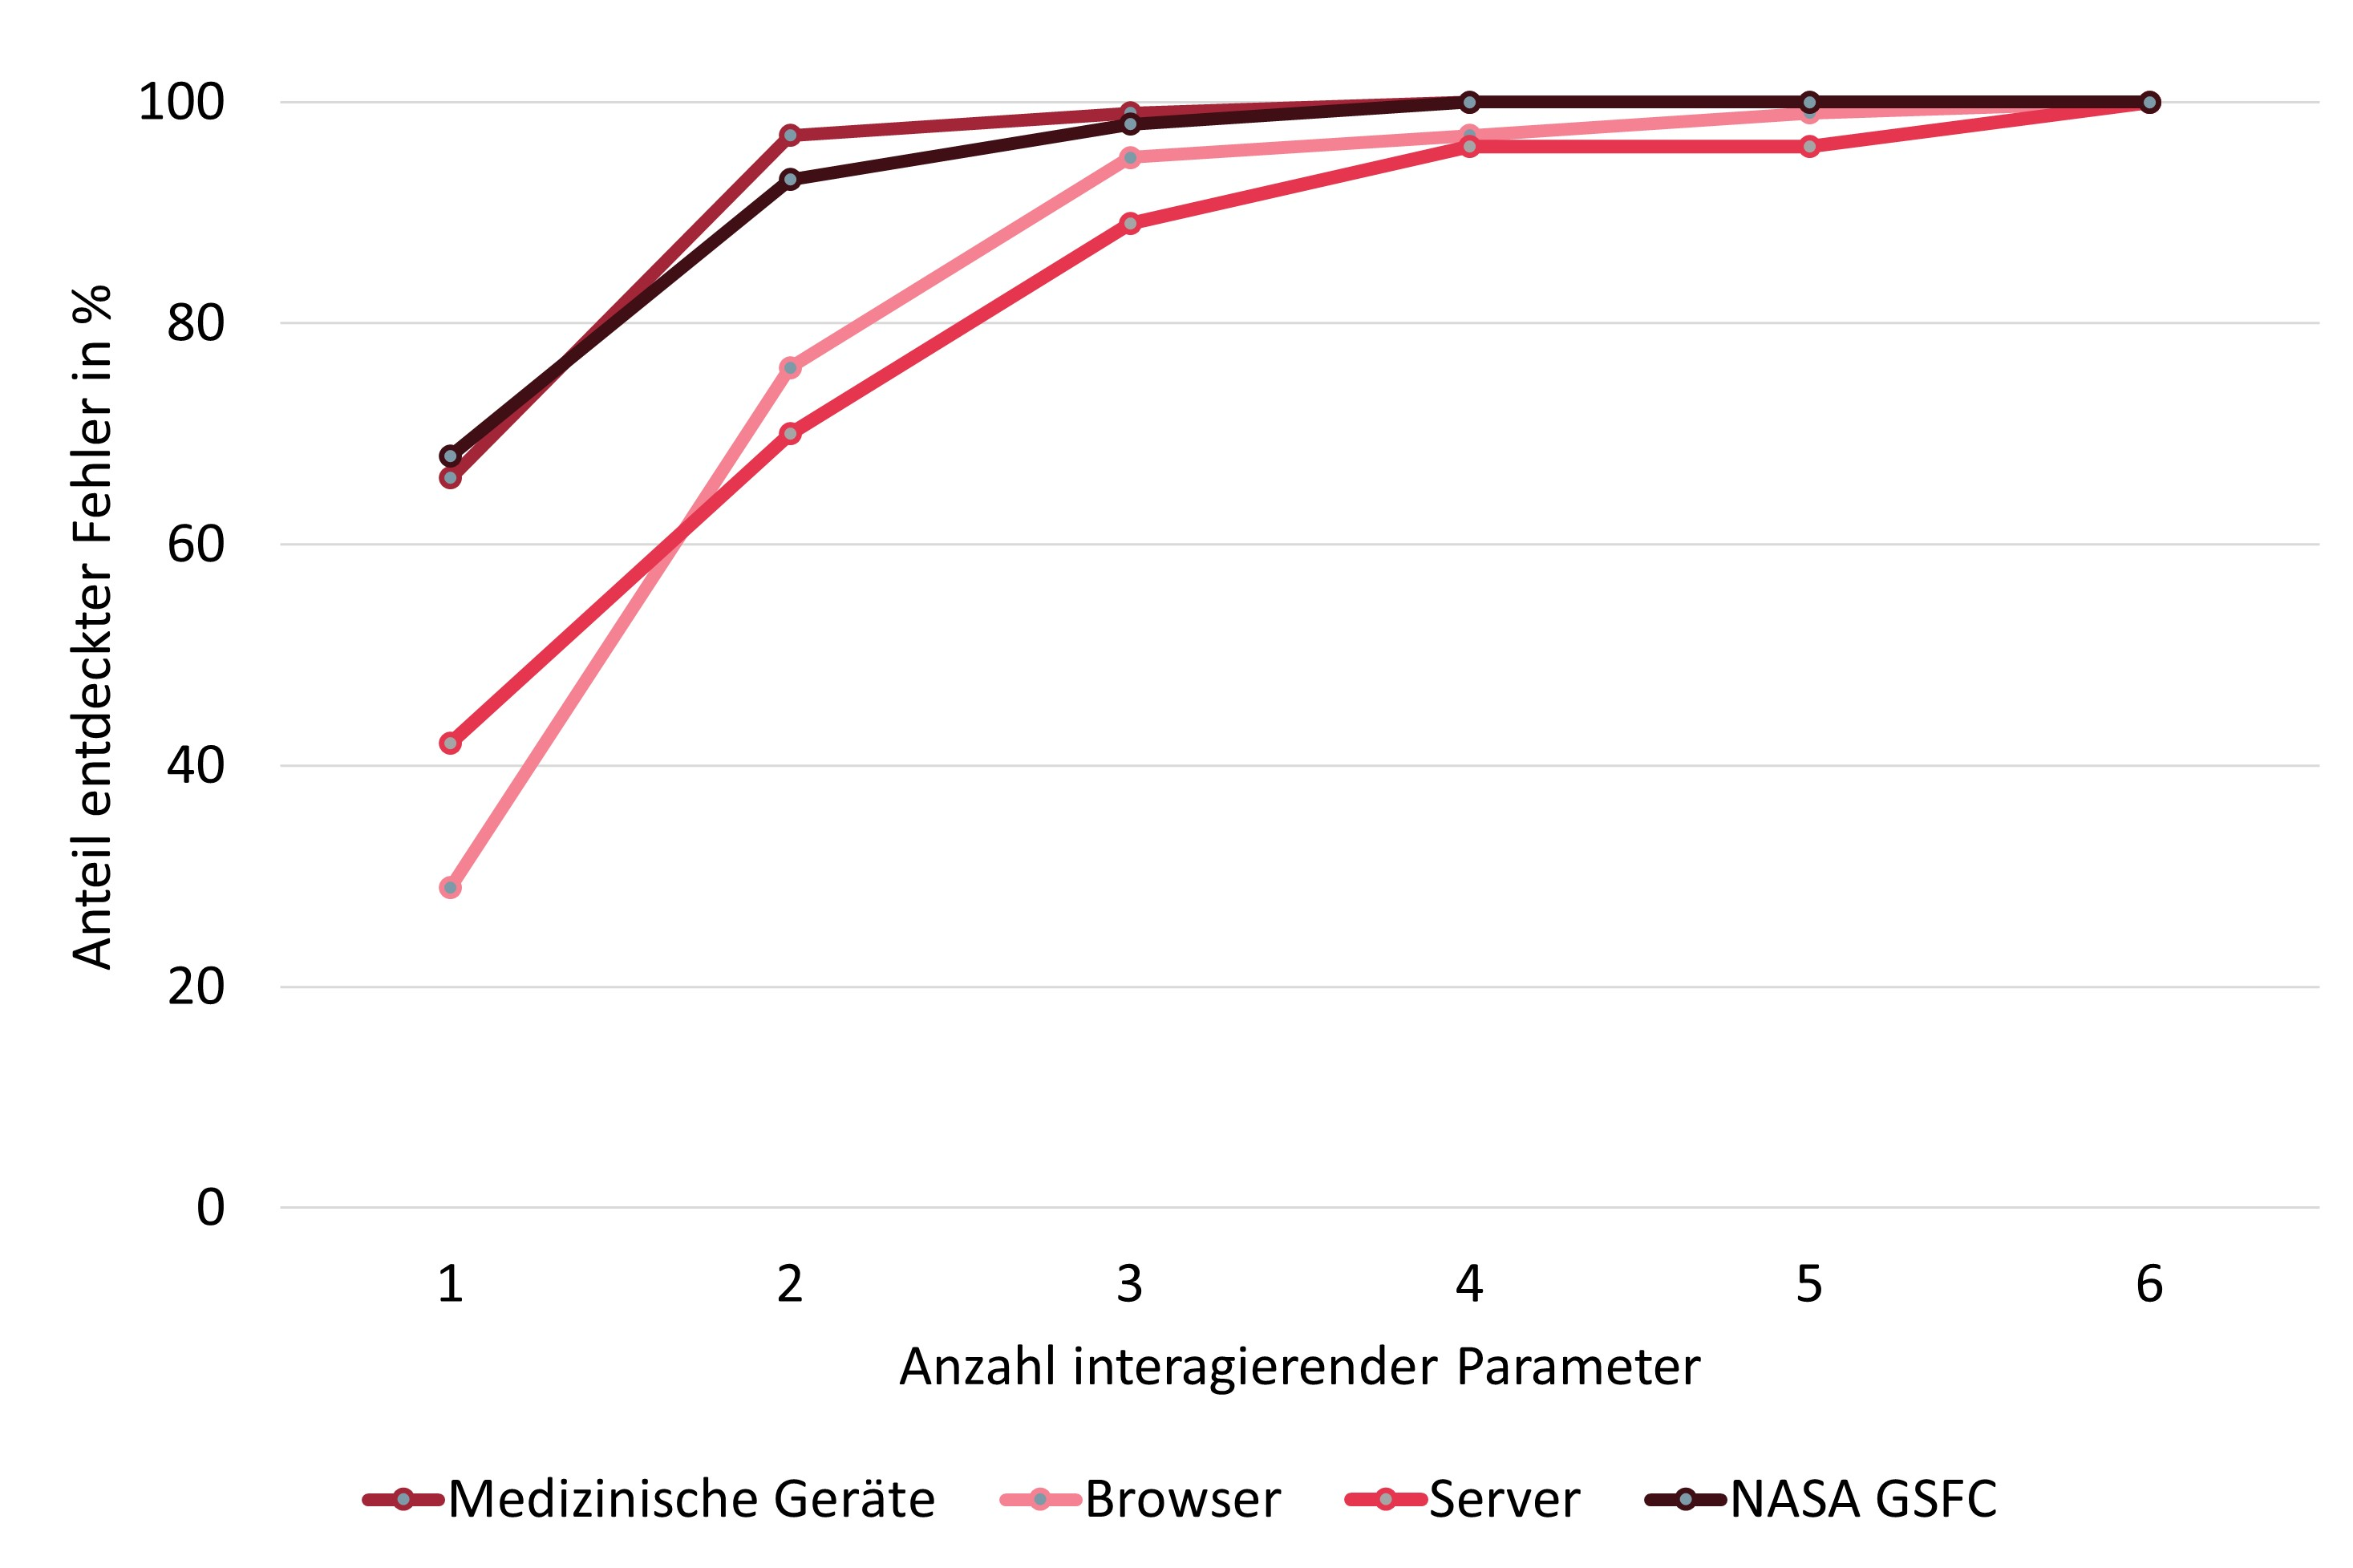
\includegraphics[width=0.6\columnwidth]{images/Fehler_Interaktion.jpg}
\caption{Fehlerverhalten verschiedener Software-Systeme nach Untersuchungen von Kuhn et al. \cite{kuhn2004error}: Die Interaktion von sechs oder weniger Parameter ist demnach für 100\% der Fehler der vier untersuchten Software-Systeme verantwortlich.}
\label{fig:fehlerInteraktion}
\end{figure}

Das folgende Beispiel in \autoref{fig:pairwise} soll die Problematik bei der Entstehung von Fehlern durch die Interaktion mehrerer Parameter verdeutlichen: Abbildung \ref{fig:pairwise} zeigt ein einfaches Beispiel angelehnt an Kuhn et al. \cite{kuhn2010practical}, bei welchem zwei Fehler unter verschiedenen Bedingungen entstehen: Fehler Nummer eins wird lediglich durch die Kombination 'Height' < 10 und 'Width' < 10 erzeugt (Codezeile 4), Fehler Nummer zwei durch die Dreierkombination 'Length' $\geq$ 10 / 'Width' $\geq$ 10 / 'Height' $\geq$ 10 (Codezeile 11). Würde man die Werte der Parameter 'Length', 'Width' und 'Height' bei der Erstellung einer Menge an Testfällen zufällig auswählen, könnte es passieren, dass diese Kombinationen durch keinen der Testfälle abgedeckt werden und somit die Fehler unentdeckt bleiben.

\begin{figure}[!htb]
\lstset{language=Java}
\begin{lstlisting}[frame=single]
				if ('Height' < 10) {
					// good code, no problem
					if ('Width' < 10) {
						// faulty code #1! BOOM!
					}
				} else if ('Height' >= 10) {
					// good code, no problem
					if ('Width' >= 10) {
						// good code, no problem
						if ('Length' >= 10) {
							// faulty code #2! BOOM!
						}
					}
				} else {
					// good code, no problem
				}
\end{lstlisting}
\caption{Beispiel für die Interaktionsproblematik beim Testen verschiedener Parameter: Bei den Kombinationen 'Height' < 10 / 'Width' < 10 und 'Length' $\geq$ 10 / 'Width' $\geq$ 10 / 'Height' $\geq$ 10 kommt es zu einem Fehlverhalten \cite{kuhn2010practical}.}
\label{fig:pairwise}
\end{figure}

Um diesem Problem zu begegnen, hat sich laut Kuhn et al. \cite{kuhn2010practical} in der Anwendungspraxis das sogenannte Pairwise-Testing etabliert, bei dem alle Kombinationen von Paaren der Eingabeparameter getestet werden. Im Beispiel von \autoref{fig:pairwise} bedeutet dies, dass alle $\binom{3}{2} = 3$ mögliche Parameterpaare mit ihren jeweils $2^2 = 4$ verschiedenen Wertekonstellationen (jeder Parameter < 10 und $\geq 10$) getestet werden sollten. Insgesamt ergibt sich dementsprechend für $t=2$ im Beispiel von \autoref{fig:pairwise} eine Anzahl von 12 zu testenden Variablen-Wert-Kombinationen. Eine Abdeckung via Pairwise-Testing würde gesichert Fehler Nummer 1 in \autoref{fig:pairwise} aufdecken, jedoch nicht garantieren, dass auch Fehler Nummer zwei entdeckt wird.

Dieses Problem löst der Ansatz des Combinatorial Testing als Erweiterung des Pairwise-Prinzips derart, dass die Zahl des zu prüfenden Interaktionsparameters variabel ist \cite{kuhn2010practical}. Konkret entspricht ein Combinatorial Testing-Ansatz mit Interaktionsparameter $t=2$ dem Pairwise-Konzept, bei $t=3$ muss jede denkbare Dreierkonstellation der Eingabeparameter mindestens in einem Testfall berücksichtigt werden. Im Beispiel aus \autoref{fig:pairwise} existieren drei verschiedenen Variablen, weshalb bei $t=3$ als einzige Parameterkonstellation diejenige Kombination bestehend aus allen drei Variablen 'Length', 'Width' und 'Height' abgedeckt werden muss. Die Gesamtzahl der zu prüfenden Wertekombinationen der drei Variablen ergibt sich aufgrund der binären Trennung der Variablen in einen Bereich > 10 und einen Bereich $\leq 10$ als $\binom{3}{3} \cdot 2^3 = 8$. Unter diesen acht acht Wertekombinationen befindet sich schließlich auch die Kombination 'Length' $\geq$ 10 / 'Width' $\geq$ 10 / 'Height' $\geq$ 10, weshalb Fehler Nummer zwei in \autoref{fig:pairwise} gesichert entdeckt werden würde.

Aus mathematischer Sicht lassen sich eine Mindest- und Maximalanzahl notwendiger Tests ($|T_{\min}|$, $|T_{\max}|$) zur zuvor beschriebenen $t$-fachen Kombinationsabdeckung (vgl. dazu auch \autoref{subsub:TAbdeckung}) anhand der Wahl des Interaktionsparameters $t$, der Anzahl $n$ aller Eingabeparameter $x_i$ und der Anzahl der möglichen Ausprägungen $y_i$ pro Parameter ermitteln: Unter der Annahme, dass der Interaktionsparameter $t$ maximal der Anzahl $n$ der vorhandenen Parameter entspricht, stellt das Produkt der $t$ größten Werte der verschiedenen Parameterausprägungen $y_i$ eine untere Schranke für die notwendigen Tests zur $t$-fachen Kombinationsabdeckung dar. Seien die Parameter also nach der Anzahl ihrer möglichen Ausprägungen geordnet, es gelte also $y_1 \geq y_2 \geq \dots \geq y_n$. Dann gilt:
\begin{gather}
|T_{\min}| = \prod_{i = 1}^{\min\{n,t\}} y_i
\end{gather}
Eine obere Schranke für die Anzahl der Tests ist unterdessen die Anzahl aller denkbaren Kombinationen der Eingabeparameter:
\begin{gather}
T_{\max} = \prod_{i=1}^{n} y_i
\end{gather}

Eine große Spannweite zwischen $|T_{\min}|$ und $|T_{\max}|$ entsteht insbesondere dann, wenn die Differenz zwischen der Anzahl der Parameter $n$ und des Interaktionsparameters $t$ groß wird. Im Gegensatz dazu liegen $|T_{\min}|$ und $|T_{\max}|$ nah beisammen, wenn $n$ und $t$ ebenfalls dicht aneinander liegen. Im Besonderen gilt für $t=n$, dass $|T_{\min}| = |T_{\max}|$. Combinatorial Testing kann seine Vorteile vor allem dann ausspielen, wenn die Differenz zwischen $|T_{\min}|$ und $|T_{\max}|$ sehr groß ist: Durch die Fokussierung auf die Interaktion von $t$ Parametern können in einem Testfall mehrere Parameterkombinationen gleichzeitig abgedeckt werden, was die Anzahl der tatsächlich benötigten Tests in Relation zu $|T_{\max}|$ sehr nahe an der unteren Schranke $|T_{\min}|$ hält.

Das in Tabelle \ref{tab:3wayInteraction} aufgeführte Beispiel aus \cite{kuhn2010practical} verdeutlicht dieses Prinzip: Die Tabelle zeigt eine mögliche Reihe an Testfällen für $n=10$ binäre ($y_i = 2 ~ \forall i = 1,\dots,n)$ Eingabevariablen A bis J bei einer Abdeckung aller Dreierkombinationen, also $t = 3$. Eine derartige Tabelle mit einer vollständigen Abdeckung aller $t$-fachen Kombinationen der Eingabeparameter nennt man im Kontext des Combinatorial Testing auch Covering Array oder Orthogonal Array. 

\begin{table}[!htb]
\begin{tabular}{|l|l|l|l|l|l|l|l|l|l|}
\hline
\cellcolor{grauinfo}A&\cellcolor{grauinfo}B&\cellcolor{grauinfo}C&\cellcolor{grauinfo}D&\cellcolor{grauinfo}E &\cellcolor{grauinfo}F&\cellcolor{grauinfo}G&\cellcolor{grauinfo}H&\cellcolor{grauinfo}I&\cellcolor{grauinfo}J\\ \hline
\cellcolor{red1}\textcolor{white}{0} & \cellcolor{red1}\textcolor{white}{0} & \cellcolor{red1}\textcolor{white}{0} & \cellcolor{red2}\textcolor{white}{0} & \cellcolor{red2}\textcolor{white}{0} & 0 & \cellcolor{red2}\textcolor{white}{0} & \cellcolor{red3}\textcolor{white}{0} & \cellcolor{red3}\textcolor{white}{0} & \cellcolor{red3}\textcolor{white}{0} \\ \hline
\cellcolor{red1}\textcolor{white}{1} & \cellcolor{red1}\textcolor{white}{1} & \cellcolor{red1}\textcolor{white}{1} & \cellcolor{red2}\textcolor{white}{1} & \cellcolor{red2}\textcolor{white}{1} & 1 & \cellcolor{red2}\textcolor{white}{1} & \cellcolor{red3}\textcolor{white}{1} & \cellcolor{red3}\textcolor{white}{1} & \cellcolor{red3}\textcolor{white}{1} \\ \hline
1 & 1 & 1 & \cellcolor{red2}\textcolor{white}{0} & \cellcolor{red2}\textcolor{white}{1} & 0 & \cellcolor{red2}\textcolor{white}{0} & \cellcolor{red3}\textcolor{white}{0} & \cellcolor{red3}\textcolor{white}{0} & \cellcolor{red3}\textcolor{white}{1} \\ \hline
\cellcolor{red1}\textcolor{white}{1} & \cellcolor{red1}\textcolor{white}{0} & \cellcolor{red1}\textcolor{white}{1} & \cellcolor{red2}\textcolor{white}{1} & \cellcolor{red2}\textcolor{white}{0} & 1 & \cellcolor{red2}\textcolor{white}{0} & \cellcolor{red3}\textcolor{white}{1} & \cellcolor{red3}\textcolor{white}{0} & \cellcolor{red3}\textcolor{white}{0} \\ \hline
\cellcolor{red1}\textcolor{white}{1} & \cellcolor{red1}\textcolor{white}{0} & \cellcolor{red1}\textcolor{white}{0} & \cellcolor{red2}\textcolor{white}{0} & \cellcolor{red2}\textcolor{white}{1} & 1 & \cellcolor{red2}\textcolor{white}{1} & 0 & 0 & 0 \\ \hline
\cellcolor{red1}\textcolor{white}{0} & \cellcolor{red1}\textcolor{white}{1} & \cellcolor{red1}\textcolor{white}{1} & 0 & 0 & 1 & 0 & \cellcolor{red3}\textcolor{white}{0} & \cellcolor{red3}\textcolor{white}{1} & \cellcolor{red3}\textcolor{white}{0} \\ \hline
\cellcolor{red1}\textcolor{white}{0} & \cellcolor{red1}\textcolor{white}{0} & \cellcolor{red1}\textcolor{white}{1} & 0 & 1 & 0 & 1 & \cellcolor{red3}\textcolor{white}{1} & \cellcolor{red3}\textcolor{white}{1} & \cellcolor{red3}\textcolor{white}{0} \\ \hline
\cellcolor{red1}\textcolor{white}{1} & \cellcolor{red1}\textcolor{white}{1} & \cellcolor{red1}\textcolor{white}{0} & \cellcolor{red2}\textcolor{white}{1} & \cellcolor{red2}\textcolor{white}{0} & 0 & \cellcolor{red2}\textcolor{white}{1} & 0 & 1 & 0 \\ \hline
0 & 0 & 0 & \cellcolor{red2}\textcolor{white}{1} & \cellcolor{red2}\textcolor{white}{1} & 1 & \cellcolor{red2}\textcolor{white}{0} & \cellcolor{red3}\textcolor{white}{0} & \cellcolor{red3}\textcolor{white}{1} & \cellcolor{red3}\textcolor{white}{1} \\ \hline
0 & 0 & 1 & 1 & 0 & 0 & 1 & 0 & 0 & 1 \\ \hline
\cellcolor{red1}\textcolor{white}{0} & \cellcolor{red1}\textcolor{white}{1} & \cellcolor{red1}\textcolor{white}{0} & 1 & 1 & 0 & 0 & \cellcolor{red3}\textcolor{white}{1} & \cellcolor{red3}\textcolor{white}{0} & \cellcolor{red3}\textcolor{white}{0} \\ \hline
1 & 0 & 0 & 0 & 0 & 0 & 0 & 1 & 1 & 1 \\ \hline
0 & 1 & 0 & \cellcolor{red2}\textcolor{white}{0} & \cellcolor{red2}\textcolor{white}{0} & 1 & \cellcolor{red2}\textcolor{white}{1} & 1 & 0 & 1 \\ \hline
\end{tabular}
\caption{Ein Covering Array für die Kombination aller Dreierkombinationen bei der Wahl von 10 binären Eingabevariablen A-J. Die verschiedenen Rotfärbungen zeigen die vollständigen Abdeckungen der Variablenkombinationen A-B-C, D-E-G und H-I-J \cite{kuhn2010practical}}.
\label{tab:3wayInteraction}
\end{table}

Würde man alle möglichen Kombinationen der 10 Variablen abdecken wollen, würde sich eine Anzahl von $T_{max} = 2^{10} = 1024$ Testfällen ergeben. Dadurch, dass nur die Kombinationen aus drei Parametern berücksichtigt werden müssen, kann die Anzahl der Testfälle auf 13 reduziert werden. Beispielhaft wird in den drei unterschiedlichen roten Farbtönen anhand der Parameterkombinationen A-B-C, D-E-G und H-I-J aufgezeigt, inwiefern mit einem Testfall mehrere Konstellationen abgedeckt werden. Im Konkreten wird durch den ersten Testfall nicht nur für die Parameterkombination A-B-C das Werte-Tupel (0,0,0) abgedeckt, sondern auch für alle $\binom{n}{t} = \binom{10}{3} = 120$ Parameterkombinationen -- unter anderem auch für die Konstellation D-E-G und H-I-J. Gleiches gilt für den zweiten Testfall und das Wertetupel (1,1,1). Testfall Nummer drei sorgt bei der Parameterkonstellation A-B-C für keine zusätzliche Abdeckung, im Falle der Kombinationen D-E-G und H-I-J werden jedoch die Wertetupel (0,1,0) und (0,0,1) neu abgedeckt. 

Dieses Vorgehen lässt sich über die 13 Testfälle in Tabelle \ref{tab:3wayInteraction} hinweg ausweiten und auf alle 120 Parameterkombinationen übertragen, sodass letztlich alle Binärkonstellationen aus drei Variablen vollständig berücksichtigt werden. Es zeigt sich also, dass in diesem Fall die tatsächlich benötigte Anzahl an Testfällen nahe an der unteren Schranke $|T_{\min}| = 2^3 = 8$ liegt, insbesondere im Vergleich zu $|T_{\max}|$.

Für den Sonderfall konstanter Ausprägungen der verschiedenen Eingabevariablen, also $y := y_i = const. ~ \forall i = 1,\dots,n$, konnten Cohen et al. \cite{cohen1997aetg} aufzeigen, dass die Anzahl der notwendigen Tests $|T|$ zur Abdeckung aller $t$-Kombinationen proportional zum Produkt aus $y^t$ und der logarithmierten Anzahl der Variablen $n$ wächst, wie \autoref{eq:proportionalität} zeigt. Insbesondere steigt die Anzahl der Testfälle bei konstanter Anzahl der Werteausprägung $y$ und konstantem Interaktionsparameter $t$ in Abhängigkeit der Anzahl der Eingabevariablen $n$ lediglich logarithmisch an.
\begin{equation}\label{eq:proportionalität}
T \sim y^t \cdot \log n
\end{equation}



\paragraph{Konfigurationstests \& Tests der Eingabewerte}

Combinatorial Testing wird im Allgemeinen in zwei Teildisziplinen unterschieden, die beide auf die zuvor aufgeführten kombinatorischen Prinzipen zurückgreifen \cite{kuhn2010practical}. Konfigurationstests fokussieren sich auf die verschiedenen Möglichkeiten, die ein Softwaresystem in Bezug auf Konfigurationsparameter einnehmen kann und welche Wechselwirkungen bei der Kombination dieser Parameter auftreten können \cite{kuhn2010practical}. Typischerweise sind damit laut Kuhn et al. \cite{kuhn2010practical} Softwaresysteme gemeint, die auf verschiedenen Betriebssystemen, verschiedenen Browsern oder unter verschiedenen Standards agieren müssen und somit eine hohe Interoperabilität erfordern. Für den Anwendungsfall dieser Arbeit ist dieser Aspekt nicht relevant.

Im Gegensatz zu den Konfigurationstests orientieren sich die Tests der Eingabewerte daran, welche konkrete Parameter in eine spezifische Komponente oder ein Softwaresystem eingegeben werden können \cite{kuhn2010practical}. Dies können beispielsweise die Auswahlfelder einer Eingabemaske wie im Anwendungsfall in \autoref{chap:anwendungsfall} oder die möglichen Variablen einer Methode wie in Abbildung \ref{fig:pairwise} betreffen. 

Eine besondere Herausforderung beim Testen der Eingabewerte besteht laut Kuhn et al. \cite{kuhn2010practical} darin, dass Eingabeparameter meist sehr viele unterschiedliche Werte annehmen können und oftmals auch Eingaben aus kontinuierlichen Zahlenbereichen möglich sind. Da die Anzahl der Tests mit der Anzahl an möglichen Werten für jede Variable exponentiell wächst (vgl. \autoref{eq:proportionalität}), würde die Berücksichtigung aller möglichen Eingaben in solchen Fällen zu einer unüberschaubaren Menge an Testfällen führen. 

Um diesem Problem zu begegnen, sollten laut Kuhn et al. \cite{kuhn2010practical} unter anderem die Strategien der Äquivalenzklassenbildung und der Grenzwertanalyse (vgl. \autoref{subsec:beispieleTests}) als Methoden zur Reduzierung der Testfälle herangezogen werden. Insgesamt empfehlen Kuhn et al. \cite{kuhn2010practical} die Anzahl verschiedener Werte beziehungsweise Klassen pro Variable auf zehn zu limitieren, da diese zur $t$-fachen Potenz in das Wachstum der Testfälle einfließt (vgl. \autoref{eq:proportionalität}). Da die Anzahl der verschiedenen Parameter $n$ nur logarithmisch auf das Wachstum der Testfälle Einfluss nimmt (vgl. \autoref{eq:proportionalität}), sei dieser Wert im Vergleich weniger kritisch zu betrachten \cite{kuhn2010practical}.

\subsection{Maße für Testabdeckung}\label{subsec:masse}

Als einer der vier hauptsächlichen Vertreter des abdeckungsbasierten Testens (vgl. \autoref{subsec:abdeckung}) erfordert das Testen der Eingabewerte wie im Falle von Combinatorial Testing Metriken, welche die Güte einer Menge von Testfällen bestimmen können.

Im Folgenden werden die wesentlichen Metriken vorgestellt, die sich im Zusammenhang mit kombinatorischen Testmethoden etabliert haben. Die ersten beiden Metriken sind dabei eher rein theoretischer Natur und spielen bei der praktischen Anwendung von Combinatorial Testing eine untergeordnete Rolle. Die Ausführungen werden durch folgendes Beispiel, angelehnt an Ammann und Offutt \cite[S. 160 ff.]{ammann2008introduction}, mit drei verschiedenen Variablen $a,b,c$, den möglichen Werten $a = \{A,B\}, b = \{1,2,3\}, c = \{x,y\}$ und der folgenden beispielhaften Menge $T$ an Testfällen in \autoref{tab:beispielMetrik} bekräftigt:
\begin{table}[h!]
\begin{tabular}{|l|l|l|}
\cellcolor{grauinfo}a   & \cellcolor{grauinfo}b & \cellcolor{grauinfo}c   \\ \hline
$A$ & 1 & $x$ \\ \hline
$A$ & 2 & $x$ \\ \hline
$A$ & 3 & $y$ \\ \hline
$B$ & 1 & $y$ \\ \hline
$B$ & 3 & $x$ \\ \hline
\end{tabular}
\caption{Testbestand $T$}.
\label{tab:beispielMetrik}
\end{table}
 
\subsubsection{Vollständige Kombinationsabdeckung}\label{subsub:VollständigeAbdeckung}

Auch wenn vollständiges Testen in verschiedener Hinsicht meist nicht durchführbar ist (vgl. Unterabschnitte \ref{subsec:testfallDesign}), lässt sich anhand der Idealvorstellung eines vollständigen Tests eine Metrik im kombinatorischen Sinne ableiten: Die vollständige Kombinationsabdeckung bezieht sich auf alle denkbaren Kombinationen der Eingabeparameter und besitzt damit die obere Schranke für Combinatorial Testing $|T_{\max}|$ als Bezugsgröße \cite[S. 160]{ammann2008introduction}. Im Beispiel der Variablen $a, b, c$ wären dies alle $2 \cdot 3 \cdot 2 = 12$ denkbaren Konstellationen. Die vollständige Kombinationsabdeckung des Testbestands $T$ liegt demnach bei $\frac{5}{12} \approx 42 \%$.

\subsubsection{Einfache Variablenabdeckung}

Die einfache Variablenabdeckung markiert in gewisser Weise die gegensätzliche Extreme zur vollständigen Abdeckung aller möglichen Kombinationen bei der vollständigen Kombinationsabdeckung: Bei der einfachen Variablenabdeckung ergibt sich die Bezugsgröße zur Bestimmung der Testfallabdeckung dadurch, dass für jede Variable isoliert betrachtet jeder mögliche Wert mindestens einmal vorkommen sollte \cite[S. 160 f.]{ammann2008introduction}. Der Testbestand $T$ erfüllt dieses Kriterium offensichtlich zu 100\%, bereits die drei Testfälle $(A, 1, x), (B, 2, y), (A, 3, x)$ würden dafür ausreichen \cite[S. 160 f.]{ammann2008introduction}. 

\subsubsection{Base Choice-Abdeckung}\label{subsub:BaseChoice}

Beim Ansatz der Base-Choice-Abdeckung wird laut Ammann und Offutt \cite[S. 162]{ammann2008introduction} für jeden Eingabeparameter eine Basiswahl festgelegt, anhand derer ein Basistestfall erstellt wird. Zusätzliche Testfälle sollten darüber hinaus durch Verändern eines einzelnen Parameters und Festhalten der Basiswerte aller anderen Parameter erzeugt werden. Im Beispiel der Variablen $a,b,c$ könnte man beispielsweise die Kombination ($A,1,x$) als Basiswahl festlegen. Dann enthält eine vollständige Base-Choice Testabdeckung die Testfälle ($A,1,x$), ($B,1,x$), ($A,2,x$), ($A,3,x$), ($A,1,y$) \cite[S. 162]{ammann2008introduction}. Tatsächlich vorhandene Testfälle in der Menge $T$ sind nur die Basiswahl selbst und $(A,2,x)$, sodass eine Testabdeckung von $\frac{2}{5} = 40 \%$ erreicht wird.

\subsubsection{$t$-fache Kombinationsabdeckung}\label{subsub:TAbdeckung}

Die $t$-fache Kombinationsabdeckung orientiert sich am Grundprinzip des Combinatorial Testing, welches in \autoref{subsec:einführungCombinatorial} vorgestellt wurde: Alle Kombinationen von $t$ verschiedenen Variablen sollten idealerweise abgedeckt werden \cite{kuhn2010practical}. So entspricht die $t$-fache Kombinationsabdeckung dem Anteil der $t$-fachen Kombinationen, die eine Menge von Testfällen abdeckt \cite{kuhn2010practical}. \autoref{tab:3wayInteraction} zeigt eine Menge von Testfällen, die eine vollständige 3-fache Kombinationsabdeckung erfüllen.
 
Wird eine Menge an Testfällen, wie in \autoref{subsec:einführungCombinatorial} beschrieben, auf Grundlage des Interaktionsparameters $t$ erstellt, erfüllt diese automatisch zu 100 \% die $t$-fache Kombinationsabdeckung \cite{kuhn2010practical}. Für $t = 2$ spricht man auch von der paarweisen Kombinationsabdeckung, da dort alle Werte der Eingabevariablen paarweise kombiniert werden \cite{kuhn2010practical}. Im Beispiel der Variablen $a,b,c$ existieren für $t = 2$ drei verschiedene 2-fach-Kombinationen $\{(a,b), (a,c), (b,c)\}$, von denen im Testbestand $T$ lediglich die Paarung $(a,c)$ alle möglichen Optionen beinhaltet. Bei $(a,b)$ fehlt die Option $(B,2)$ und bei $(b,c)$ die Option $(2,y)$. Dies entspricht einer Abdeckung von $\frac{1}{3} \approx 33,3 \%$. 

Allgemein entspricht die Anzahl der zu prüfenden $t$-fachen Kombinationen $K_t$ dem Binomialkoeffizienten aus der Anzahl der Eingabeparameter und dem Interaktionsparameter $t$:
\[
K_t = \binom{n}{t}
\]

Um festzustellen, ob eine der $\binom{n}{t}$ Parameterkombinationen vollständig in einem Testdatensatz vorhanden ist, müssen alle Variablen-Wert-Konfigurationen für jeden Parameter geprüft werden. Beim Testbestand $T$ sind dies genau 16 Stück.

\subsubsection{$(t+k)$-fache Kombinationsabdeckung}\label{subsub:tPlusKAbdeckung}

Jede Menge an Testfällen, die einen hohen Anteil einer $t$-fachen Kombinationsabdeckung aufweist, wird auch einen gewissen Anteil einer $(t+k)$-fachen Kombinationen abdecken \cite{kuhn2010practical}. Insbesondere dann, wenn verschiedene Mengen von Testfällen auf Basis einer $t$-fachen Kombinationsabdeckung erstellt wurden und somit in dieser Hinsicht eine Abdeckung von 100\% erfüllen, wird laut Kuhn et al. \cite{kuhn2010practical} mittels der$(t+k)$-fachen Kombinationsabdeckung eine Vergleichbarkeit ermöglicht: Neben der absoluten Anzahl an Testfällen, welche zur vollständigen Abdeckung vonnöten sind, können unter anderem die $(t+1)$-fache oder $(t+2)$-fache Kombinationsabdeckung als Vergleichskriterium zwischen zwei Mengen von Testfällen herangezogen werden. Der Testbestand $T$ besitzt, wie zuvor aufgeführt, eine $2$-fache Kombinationsabdeckung von ungefähr 33,3 \%. Prüft man nun die Abdeckung bezüglich $(t+1) = 3$, ergibt sich eine Abdeckung von 0\%, da die einzig vorhandene Dreierkonstellation $(a,b,c)$ offensichtlich nicht vollständig vorhanden ist.  

\subsubsection{Variablen-Wert-Abdeckung}\label{subsub:variablenWert}

Bei der Betrachtung der $t$-fachen Kombinationsabdeckung wird für jeden Eingabeparameter $x_i$ lediglich geprüft, ob alle $t$-fachen Kombinationen abgedeckt sind, und dabei nicht berücksichtigt, wie viele Werte-Kombinationen zu einer vollständigen Abdeckung im Hinblick auf die jeweiligen Variablen $x_i$ fehlen würden: Die Variablen-Wert-Abdeckung greift laut Kuhn et al. \cite{kuhn2010practical} diese Problematik auf und prüft für jede $t$-fache Variablenkombination den Anteil der abgedeckten Kombinationsmöglichkeiten der möglichen Werte. Wird beispielsweise $t=2$ gewählt, existieren bei binären Eingabeparametern vier verschiedene Kombinationsmöglichkeiten für jedes Paar der Parameter.
  

Der Testbestand $T$ besitzt für $t=2$ die $K_t = \binom{n}{t} = 3$ verschiedenen Parameterpaarungen $(a,b), (a,c), (b,c)$. Für das Paar $(a,b)$ existieren aufgrund der Anzahl der möglichen Ausprägungen von $a$ und $b$ genau $2 \cdot 3 = 6$ verschiedene Wertekonstellationen, dasselbe gilt für das Parameterpaar $(b,c)$. Die Paarung $(a,c)$ besitzt $2 \cdot 2 = 4$ vier mögliche Wertekonstellationen, da beide Parameter zwei Ausprägungen besitzen. Insgesamt ergibt sich eine Anzahl von 16 verschiedenen Variablen-Wert-Konstellationen, die für eine vollständige Variablen-Wert-Abdeckung abzuprüfen sind. Die vier Kombinationen von $(a,c)$ sind vollständig vorhanden, bei $(a,b)$ und $(b,c)$ fehlt jeweils eine der sechs Optionen. Dementsprechend liegt die Variablen-Wert-Konfiguration hier bei $\frac{14}{16} \approx 87,5 \%$. Zum Vergleich: Der Wert der 2-fachen Kombinationsabdeckung liegt bei 33,3\%.

\begin{comment}
Seien wie in \autoref{sec:combinatorialTesting} $n$ die Anzahl der verschiedenen Parameter $x_i$, $y_i$ die zu einem Eingabeparameter $x_i$ gehörende Anzahl an verschiedenen Werten und $t$ der Interaktionsparameter. Allgemein lässt sich dann die Anzahl aller möglichen Variablen-Wert-Kombinationen $V_{t}$ folgendermaßen bestimmen:
\begin{gather*}
V_t = \sum_{i = 1}^{n-t+1} y_i \cdot \sum_{Z \in U_i} \prod_{z \in Z} z ~\text{ wobei} \\
U_i = \{U ~ | ~ U \in \mathcal{P}(Y_i) \land |V| = t-1\}  ~\text{ und} \\
Y_i = \{y_j ~ | ~ x_j \text{ ist Eingabeparameter mit $y_j$ verschiedenen Werten} \land i < j\}  
\end{gather*}

Diese Berechnungsvorschrift ist wie folgt zu verstehen: Es wird über die Eingabewerte $x_i$ iteriert und dabei für jeden Parameter die verbleibende Restanzahl an $t$-fachen Kombinationen ermittelt. Der Abbruch der Iterationen erfolgt bereits bei $n-t+1$, da ab dort keine weiteren Kombinationen möglich sind. 

Konkret entspricht $Y_i$ der Menge, welche die Anzahl der unterschiedlichen Werte $y_i$ der noch nicht bearbeitenden $x_i$ beinhaltet - also diejenigen $x_j$ für die $j > i$ gilt. Im Beispiel der Variablen $a,b,c$ wäre dies bei der Wahl von $x_1 = a$ die Menge $\{2,3\}$. Aus dieser Menge werden nun in $U_i$ alle Kombinationen, die gemeinsam mit dem aktuell ausgewählten $x_i$ eine $t$-fache Kombination darstellen können, ausgewählt. Dies geschieht über die Bildung der Potenzmenge und der Prüfung, ob die Mächtigkeit einer Teilmenge $t-1$ entspricht. $x_i$ selbst sorgt dafür, dass aus der Zahl $t-1$ eine $t$-fache Kombination folgt. Jede Menge $Z$ in $U_i$ beinhaltet dann $t-1$ Zahlen, welche für die mögliche Anzahl verschiedener Parameterwerte stehen. Gemeinsam mit den $y_i$ möglichen Eingabewerten für den \glqq Haupteingabeparameter\grqq{} zu diesem Zeitpunkt, $x_i$, ergeben sich dann für die betroffene Menge $Z$ genau $y_i \cdot \prod_{y \in Z} y$ t-fach-Kombinationen aus $x_i$ und den $x_j$, die zu den $y_j \in Z$ gehören. Abschließend gilt es die Summe über alle Kandidaten $Z$ in $U_i$ zu bilden, ehe die nächste Iteration folgt.

\end{comment}


\subsubsection{$(p,t)$-Vollständigkeit}\label{subsub:pTVollständigkeit}

Über die Variablen-Wert-Konfiguration hinaus definieren Kuhn et al. \cite{kuhn2010practical} die $(p,t)$-Vollständigkeit als ein weiterführendes Maß zur Quantifizierung der kombinatorischen Testgüte. Die $(p,t)$-Vollständigkeit wird dabei definiert als der Anteil der $K_t = \binom{n}{t}$ Parameterkombinationen, deren Variablen-Wert-Konfigurationsabdeckung mindestens $p$ überschreiten.

Im Testbestand $T$ fehlen in Bezug auf $t=2$ einzig bei den Parameterpaaren $(a,b)$ und $(b,c)$ eine der jeweils sechs Kombinationen, sodass diese Kombinationen für $p \leq \frac{5}{6}$ die Anforderung an die $(p,t)$-Vollständigkeit erfüllen. Zudem erfüllt die Kombination $(a,c)$ aufgrund der vollständigen Variablen-Wert-Abdeckung für jedes $p$ die $(p,t)$-Vollständigkeit. Wählt man also beispielsweise $p=75\%$, liegt die (p,t)-Vollständigkeit des Testbestands $T$ insgesamt bei 100\%, da alle drei Parameterpaare die Variablen-Wert-Konfigurationsabdeckung von $75\%$ überschreiten.

\subsection{Algorithmen zur Testfallerzeugung}\label{subsec:algo}

In der Vergangenheit wurden verschiedene Algorithmen entwickelt, die eine Menge an Testfällen mit kombinatorischer Abdeckung, also im Wesentlichen Covering Arrays, erstellen können. Khalsa und Labiche \cite{khalsa2014orchestrated} konnten in einer Metaanalyse im Jahr 2014 75 verschiedene Algorithmen und Tools entdecken, die auf unterschiedliche Art und Weise kombinatorische Methoden zur Testfallerzeugung anwenden. Diese Arbeit markiert die zum aktuellen Zeitpunkt größte Übersicht über die vorhanden Algorithmen und Tools zu Combinatorial Testing.

Laut Khalsa und Labiche \cite{khalsa2014orchestrated} lassen sich die Algorithmen zur Erstellung von Testmengen bei Combinatorial Testing zwei grundlegenden Kategorien zuordnen, den Test-basierten und Parameter-basierten Methoden: Parameter-basierte Algorithmen berücksichtigen laut Khalsa und Labiche \cite{khalsa2014orchestrated} zunächst nur $t$ Eingabeparameter und erstellen für diesen Fall eine Testmenge mit vollständiger $t$-facher Abdeckung. Anschließend werden die Testfälle dann so erweitert, dass diese mit Werten der $n-t$ fehlenden Parametern belegt werden. Falls notwendig, werden weitere Testfälle auf dem Weg zu einer vollständigen $t$-fachen Abdeckung ergänzt. Diese Erweiterung kann beispielsweise als Greedy-Verfahren oder anhand rekursiver, algebraischer Methoden vorgenommen werden \cite{khalsa2014orchestrated}. Ein Beispiel hierfür ist der IPOG-Algorithmus (vgl. \autoref{subsub:ipog}).

Im Gegensatz dazu wird bei der Test-basierten Variante ein Testfall derart erzeugt, dass dieser in einem Schritt möglichst viele einfache $t$-fache Konfigurationen (vgl. \autoref{subsec:masse}) abdeckt und dabei im Vergleich zu den Parameter-basierten Algorithmen alle Eingabeparameter berücksichtigt \cite{khalsa2014orchestrated}. Erweiterungsschritte für nicht berücksichtigte Parameter wie im Falle der Parameter-basierten Algorithmen sind hier nicht notwendig. Beispiel für ein Test-basiertes Verfahren ist der AETG-Algorithmus (vgl. \autoref{subsub:aetg}). 

Ungeachtet dieser Unterteilung konnten Khalsa und Labiche \cite{khalsa2014orchestrated} fünf verschiedene Algorithmen-Klassen den vorhanden Combinatorial Testing Tools und Algorithmen zuordnen:
\begin{itemize}
\item Greedy-Verfahren: Eine optimale Lösung in Bezug auf eine Bewertungsfunktion versucht man bei Greedy-Verfahren durch Iterationsschritte lediglich auf Basis der lokal verfügbaren Informationen zu finden \cite[S. 185]{schoening2001algorithmik}. In Bezug auf Combinatorial Testing bedeutet dies, dass ausgehend von einer bestehenden Menge an Testfällen weitere Testfälle möglichst viele der noch nicht berücksichtigten Kombinationen abdecken \cite{khalsa2014orchestrated} sollten. Greedy-Verfahren machen den Großteil (53 \%) der von Khalsa und Labiche \cite{khalsa2014orchestrated} entdeckten Algorithmen und Tools für Combinatorial Testing aus.
\item Meta-Heuristiken: Im Allgemeinen wird bei heuristischen Algorithmen versucht, das Auffinden einer optimalen Lösung eines Optimierungsproblems durch Zuhilfenahme \glqq problem-spezifischer Informationen\grqq{} \cite[S. 319]{schoening2001algorithmik}, sogenannten \glqq Heuristiken\grqq{}, zu beschleunigen \cite[S. 319]{schoening2001algorithmik}. Im Konkreten werden im Kontext von Combinatorial Testing unter anderem die Methoden der genetischen Algorithmen, der Partikelschwarmoptimierung oder des Simulated Annealing verwendet \cite{khalsa2014orchestrated}. Im Vergleich zu Greedy-Methoden sind laut Khalsa und Labiche \cite{khalsa2014orchestrated} Meta-Heuristiken meist langsamer in ihrer Ausführung, liefern aber häufig bessere Lösungen im Sinne einer kleineren Menge an benötigten Testfällen.
\item Adaptive Random-/Adhoc-Verfahren: Diese Kategorie der Algorithmen-Klassen für Combinatorial Testing fokussiert sich im Grundsatz auf eine zufallsgesteuerte Erzeugung von Testfällen \cite{khalsa2014orchestrated}. Adhoc-Verfahren erzeugen laut Khalsa und Labiche \cite{khalsa2014orchestrated} Testfälle auf Grundlage einer zuvor angenommenen Wahrscheinlichkeitsverteilung. Bei Adaptive Random-Methoden wird durch ein Distanzmaß, beispielsweise dem Hamming-Abstand, gewährleistet, dass die erzeugten Testfälle sich nicht zu stark überschneiden und so eine geringe Menge an Testfällen zur $t$-fachen Abdeckung ausreicht \cite{khalsa2014orchestrated}. 
\item Algebraische Verfahren: Algebraische Verfahren erzeugen Testfälle anhand einer vorgegebenen mathematischen Funktion oder vordefinierten mathematischen Regeln \cite{khalsa2014orchestrated}. Unter anderem werden dabei auch rekursive Methoden verwendet, um die Komplexität der Problematik auf kleinere Teilprobleme zu reduzieren.
\item Hybride Methoden: Die Konzepte verschiedener zuvor aufgeführten Konzepte zu vereinen, steckt als Grundidee hinter den hybriden Verfahren \cite{khalsa2014orchestrated}. Ein Beispiel hierfür ist der modifizierte IPOG-D-Algorithmus (vgl. \autoref{subsub:ipog}).
\end{itemize}

Neben den unterschiedlichen Strategien zur Testfallerzeugung existieren zwischen den verschiedenen Algorithmen und Tools laut Khalsa und Labiche \cite{khalsa2014orchestrated} wesentliche Unterschiede unter anderem in der maximal unterstützten Höhe des Interaktionsparameters $t$ und der Möglichkeit, Bedingungen an das Testsystem zu stellen, sodass gewisse kombinatorische Möglichkeiten ausgeschlossen werden können. Zudem besitzt nicht jeder Algorithmus die Möglichkeit, sogenannte Mixed Covering Arrays abzudecken, also Testfälle, bei denen jeder Eingabeparameter eine unterschiedliche Anzahl an Werten einnehmen kann \cite{khalsa2014orchestrated}.

Im Folgenden werden beispielhaft relevante Vertreter der Algorithmen zur Erstellung von Covering Arrays vorgestellt. Diese decken nur einen Bruchteil der existierenden Methoden zur Testmengen-Erstellung dar und fokussieren sich demnach insbesondere auf diejenigen Algorithmen, die im Rahmen dieser Arbeit eine wichtige Rolle spielen.

\subsubsection{AETG}\label{subsub:aetg}

Als mitunter erste Wissenschaftler überhaupt beschäftigten sich Cohen et al. \cite{cohen1997aetg} 1997 mit den Methoden des Combinatorial Testing und der Frage, wie auf effiziente Art und Weise Covering Arrays erstellt werden können. Der von Cohen et al. \cite{cohen1997aetg} entwickelte Algorithmus und das zugehörige AETG (Automatic Efficient Test Generator) System waren über lange Zeit das de facto Standardtool in Bezug auf kombinatorische Testmethoden. Das kommerzielle AETG System ist jedoch in seiner ursprünglichen Form nicht mehr verfügbar, soll aber aufgrund seiner historischen Bedeutung kurz vorgestellt werden.

Der AETG-Algorithmus ist ein Greedy-Verfahren, das grundsätzlich eine beliebige Höhe des Interaktionsparameters $t$ abdecken kann \cite{cohen1997aetg}. Die tatsächliche Realisierung des AETG-Systems wurde jedoch lediglich für eine paarweise Kombinationsabdeckung ($t = 2$) entwickelt \cite{khalsa2014orchestrated}. Darüber hinaus besitzt das AETG System die Möglichkeit unerwünschte Kombinationen durch explizite Angabe von \glqq verbotenen Tupeln\grqq{} auszuschließen \cite{cohen1997aetg, khalsa2014orchestrated}.

Der konkrete Algorithmus, der als Test-basierter Algorithmus einzustufen ist, soll im Folgenden kurz erläutert werden. Eine detailliertere Beschreibung der Vorgehensweise lässt sich bei Cohen et al. \cite{cohen1997aetg} finden. 

Seien $n$ verschiedene Eingaparameter $x_1, \dots, x_n$, die Anzahl der verschiedenen Ausprägungen der Eingaparameter  $y_1, \cdots, y_n$ gegeben und die verschiedenen Ausprägungen des i-ten Eingabeparameters als $z_{ij}$ mit $j = 1,...,y_i$ definiert. Unter der Annahme, dass bereits $r$ Testfälle erzeugt wurden, entsteht der $(r+1)$-te Testfall durch das folgende Prinzip:
\begin{enumerate}
\item Zufällig wird ein Parameter $x_{\tilde{i}}$ gewählt und für diesen Parameter die Ausprägung $z_{\tilde{i}\tilde{j}}$ ermittelt, die bisher durch die wenigsten $t$-fachen Kombinationen abgedeckt ist. Anschließend werden die übrigen Parameter zufällig geordnet: Sei $i_1, \cdots, i_{n-1}$ die zufällige erzeugte Indexfolge von 1 bis $n-1$. Dann werden die Parameter als Folge $a_1 := x_{i_1}, a_2 := x_{i_2}  \dots, a_{n-1} := x_{i_{n-1}}$ geordnet.
\item Nun wird für jeden Parameter der erstellten Folge $a_i$ der Wert des $(r+1)$-ten Testfalls folgendermaßen bestimmt: Angenommen es seien bereits die Werte für $a_1, \dots a_j$ festgelegt, dann ergibt sich der Wert des Parameters $a_{j+1}$ dadurch, dass für jeden möglichen Wert von $a_{j+1}$ geprüft wird, wie viele neue $t$-fachen Überdeckungen in Kombination mit den bereits gewählten Werten von $a_1, \dots, a_j$ entstehen würden. Davon wird schließlich das Maximum ausgewählt.
\end{enumerate}

Dieses Vorgehen soll anhand des Beispiels aus \autoref{subsec:masse} und des Testbestands $T$ (vgl. \autoref{tab:beispielMetrik}) mit den drei verschiedenen Variablen $\{a,b,c\} ~ (\hat{=} ~ \{x_1, x_2, x_3\})$ und den möglichen Werten $a \in \{A,B\} ~ (\hat{=} ~ \{z_{11}, z_{12}\}), b \in \{1,2,3\} ~ (\hat{=} ~ \{z_{22}, z_{22}, z_{23}\}), c \in \{x,y\} ~ (\hat{=} ~ \{z_{31}, z_{32}\})$ verdeutlicht werden. Der Interaktionsparameter wird auf $t=2$ festgesetzt. 

Angenommen, es wurde bereits der erste Testfall des Testbestands $T$ $(A,1,x)$ erzeugt, dann soll nun erläutert werden, wie AETG einen zweiten Testfall erstellt: Im ersten Schritt des Algorithmus wird zunächst zufällig einer der drei Parameter gewählt, beispielsweise $b$. Bisher wurden für diesen Parameter die Paare $(A,1)$ und $(1,x)$ abgedeckt, sodass für die Ausprägung $z_{21} = 1$ bereits zwei der insgesamt 12 verschiedenen Kombinationen der Variablen $b$ abgedeckt wurden. Die Ausprägungen $z_{22} = 2$ und $z_{23} = 3$ wurden bisher noch nicht abgedeckt, eine von beiden wird somit für den nächsten Testfall als Grundlage $z_{\tilde{i}\tilde{j}}$ gewählt. Dies soll $z_{22} = 2$ sein. Anschließend erfolgt die zufällige Ordnung der verbleibenden Variablen in einer Folge, diese soll $a_1 := a$ und $a_2 := c$ entsprechen.

Im zweiten Schritt des Algorithmus wird zunächst für $a_1 = a$ der Wert mit der maximalen, zusätzlichen Abdeckung gewählt. Da für die Variable $a$ bisher lediglich die Paarung $(A,1)$ abgedeckt wird, würde sowohl die Wahl des Wertes $A$ als des Wertes $B$ eine zusätzliche Abdeckung der Parameter $a$ und $b$ bedeuten. Angenommen, an dieser Stelle wird der Wert $A$ gewählt, ergibt sich im folgenden, identischen Schritt für Parameter $a_2 = c$ die Wahl des Wertes $y$ zur Vervollständigung des Testfalls: Eine Ergänzung durch den Wert $x$ würde zu der Wertepaarung $(A,x)$ führen, die jedoch bereits über den ersten Testfall abgedeckt ist. Damit ist die Anzahl der zusätzlichen $t$-fachen Überdeckung bei Wahl des Wertes $y$ höher, weshalb dieser in diesem Schritt des AETG-Algorithmus den Vorzug erhält. Als neuer Testfall ergibt sich also das Wertetupel $(A, 2, y)$.

\subsubsection{IPOG}\label{subsub:ipog}

Der IPOG-Algorithmus (In-Parameter-Order-Generalization) stellt als Parameter-basierte Variante ein alternatives Greedy-Verfahren zum AETG-Algorithmus dar, das insbesondere im ACTS-Tool (vgl. \autoref{subsub:acts}) eine wesentliche Rolle spielt. IPOG wurde 2007 von Lei et al. \cite{lei2008ipog} vorgestellt und stellt eine Erweiterung des allgemeinen IPO-Algorithmus \cite{lei1998parameter} dar, der die grundlegende Idee der Parameter-basierten Erzeugung in einfachster Form für paarweises Testen ($t=2$) umsetzt.

Sei $n$ die Anzahl der verschiedenen Eingabeparameter, $x_i$, $y_i$ die Anzahl der möglichen Ausprägungen des Parameters $x_i$, $t$ der Interaktionsparameter und $T$ die aus dem Algorithmus resultierende Menge an Testfällen. Zudem seien die Parameter nach der Anzahl ihrer möglichen Ausprägungen geordnet, es gelte also $y_1 \geq y_2 \geq \dots \geq y_n$. Dann funktioniert der IPOG-Algorithmus folgendermaßen. Eine vollständige Beschreibung inklusive Pseudocode lässt sich bei Lei et al. \cite{lei2008ipog} nachlesen:
\begin{enumerate}
\item Die Menge der ausgegebenen Testfälle $T$ wird als leere Menge initialisiert. Dann wird zunächst für die ersten $t$ Parameter $x_1,\dots,x_t$ eine vollständige Kombinationsabdeckung (vgl. \autoref{subsub:VollständigeAbdeckung}) gebildet und in die Menge $T$ eingefügt. Falls $n > t$ folgt nun eine iterative Erweiterung der Testfälle in $T$ für jeden Parameter $x_j$ mit $t < j \leq n$, also die Parameter, die unter den ersten $t$ Parametern nicht dabei waren.
\item In jeder Iteration wird für den aktuellen Parameter $x_i$ mit $t < j \leq n$ eine Menge $\pi$ berechnet, die alle $t$-fachen Kombinationen mit den bereits berücksichtigten Parametern $j$ mit $1 \leq j < i$ beinhaltet, die abgedeckt werden müssen. Man beachte, dass die Testmenge $T$ bei der $i$-ten Iteration bereits eine vollständige $t$-fache Abdeckung für die Parameter $x_1,\dots,x_{i-1}$ besitzt. Die fehlenden Testfälle zur Abdeckung von $x_1,\dots,x_i$ werden nun in zwei Schritten vorgenommen, die Lei et al. als \glqq horizontales' und 'vertikales Wachstum\grqq{} \cite{lei2008ipog} bezeichnen.
\item Beim horizontalen Wachstum wird für jeden bereits existierenden Testfall ein zusätzlicher Wert für den Parameter $x_i$ angefügt und dabei jener Wert ausgewählt, der in der zuvor erstellten Kombinationsmenge $\pi$ die meisten Kombinationen abdecken kann. Neu abgedeckte Wertekombinationen werden stets aus $\pi$ entfernt.

Bei der folgenden vertikalen Erweiterung wird für alle noch verbleibenden $t$-fachen Kombinationen in der Menge $\pi$ grundsätzlich ein neuer Testfall erstellt, bei dem die Werte der aktuell gewählten Parameter der $t$-fach Kombination durch die jeweiligen Werte der $t$-fach Kombination vorgegeben werden und alle anderen Werte auf sogenannte \glqq Don't Cares\grqq{} gesetzt werden. Dies soll gewährleisten, dass die Werte der nicht betroffenen Variablen für weitere Erweiterungen flexibel bleiben. Denn neben der Erzeugung eines Testfalls wird stets bei jeder Iteration des vertikalen Wachstums geprüft, ob eine Kombination durch Anpassungen derartiger \glqq Don't Cares\grqq{} abgedeckt werden kann und somit kein neuer Testfall erstellt werden muss. Trifft dies zu, werden die \glqq Don't Cares\grqq{} durch die passenden Werte der jeweiligen Parameter ersetzt und werden gewissermaßen zu \glqq Do Cares\grqq{}.
\end{enumerate}

Verdeutlicht wird dieses Verfahren anhand des Beispiels aus \autoref{subsec:masse} mit den drei verschiedenen Variablen $a,b,c$ und den möglichen Werten $a \in \{A,B\}, b \in \{1,2,3\}, c \in \{x,y\}$: Der Interaktionsparameter sei auf $t = 2$ festgesetzt: Im ersten Schritt des Algorithmus werden die Parameter der Anzahl ihrer Ausprägungen nach absteigend sortiert. Dies ergibt die Folge $(y_1 = b, y_2 = a, y_3 = b)$ ($b$ und $a$ könnten vertauscht werden). Anschließend wird eine Tabelle zur vollständigen Kombinationsabdeckung der ersten $t=2$ Parameter erstellt, die in \autoref{tab:ipogTabelle} auf der linken Seite dargestellt ist.

\begin{table}[!htb]
    \begin{minipage}{0.25\linewidth}
      \raggedleft
        \begin{tabular}{|l|l|}
			\cellcolor{grauinfo}a   & \cellcolor{grauinfo}b  \\ \hline
			$A$ & 1 \\ \hline
			$A$ & 2 \\ \hline
			$A$ & 3 \\ \hline
			$B$ & 1 \\ \hline
			$B$ & 2 \\ \hline
			$B$ & 3 \\ \hline
		\end{tabular}
    \end{minipage}%
	\begin{minipage}{0.35\linewidth}
      \centering
		
\includegraphics[width=0.4\linewidth]{images/arrow.jpg}
    \end{minipage} 
    \begin{minipage}{0.25\linewidth}
      \raggedright
        \begin{tabular}{|l|l|l|}
			\cellcolor{grauinfo}a   & \cellcolor{grauinfo}b & \cellcolor{grauinfo}c   \\ \hline
			$A$ & 1 & $x$ \\ \hline
			$A$ & 2 & $y$ \\ \hline
			$A$ & 3 & $x$ \\ \hline
			$B$ & 1 & $y$ \\ \hline
			$B$ & 2 & $x$ \\ \hline
			$B$ & 3 & $y$ \\ \hline
		\end{tabular}
    \end{minipage} 
    \caption{Struktur des IPOG-Algorithmus anhand des Beispiels aus \autoref{subsec:masse}) und $t=2$: Zunächst wird für $t$ Parameter eine Tabelle mit einer vollständigen Kombinationsabdeckung erstellt (linke Seite). Anschließend wird diese Tabelle horizontal (rechte Seite) und vertikal erweitert. Im Beispiel entfällt die vertikale Erweiterung, da bereits nach der horizontalen Erweiterung alle Variablenpaare vollständig abgedeckt sind.}
	\label{tab:ipogTabelle}
\end{table}

Im nächsten Schritt des IPOG-Algorithmus wird nun die Menge $\pi$ ermittelt, die alle noch nicht abgedeckten Wertekombinationen beinhaltet. Im Beispiel gilt: \[\pi = \{(A,x), (A,y), (B,x), (B,y), (1,x), (2,x), (3,x), (1,y), (2,y), (3,y)\}\]
Im Folgenden werden die Testfälle der zuvor erstellten vollständigen Kombinationsabdeckung für $t=2$ (vgl. linke Seite \autoref{tab:ipogTabelle}) \glqq horizontal\grqq{} erweitert. Für den ersten Testfall $(A,1)$ ergibt sich sowohl für den Wert $c=x$ als auch $c=y$ eine zusätzliche Abdeckung von zwei Kombinationen. In diesem Beispiel soll an dieser Stelle der Wert $c=x$ gewählt werden. Für den nächsten Testfall wird nun der Wert $c=y$ gewählt, da dieser zwei Kombinationen neu abdecken würde und $c=x$ nur einen. Dieses Vorgehen wird für alle sechs Testfälle der anfänglichen Tabelle mit vollständiger Kombinationsabdeckung wiederholt. Die rechte Seite der \autoref{tab:ipogTabelle} zeigt das Resultat. Im Beispiel sind damit alle drei Paarungen der drei Variablen $a,b,c$ vollständig abgedeckt, sodass der vertikale Erweiterungsschritt des IPOG-Algorithmus entfällt.


\hspace{1cm} Der IPOG-Algorithmus zählt während seiner Ausführung alle denkbaren $t$-fachen Kombinationen auf und besitzt laut Lei et al. \cite{lei2008ipog} die Zeitkomplexität von $ O(y_1^{t+1} \cdot n^{t-1} \cdot \log n)$, wobei $n, t$ und $y_1$ den zuvor eingeführten Definitionen entsprechen. Dementsprechend ist der allgemeine IPOG-Algorithmus insbesondere bei sehr großen Systemen ineffektiv \cite{lei2008ipog}, was zu verschiedenen Erweiterungen des Algorithmus führte. 

Der IPOG-D-Algorithmus \cite{lei2008ipog} vereint die Methoden des allgemeinen IPOG-Algorith- mus und eines algebraisch-rekursiven Ansatzes, um bei der Erstellung der Testfälle nicht alle Kombinationsmöglichkeiten explizit aufzählen zu müssen. Im Konkreten wird dabei der erste Schritt des zuvor erläuterten IPOG-Algorithmus, also die initiale Erstellung einer $t$-fachen Abdeckung für die ersten $t$ Parameter, mittels einer rekursiven Methode optimiert. Ein Verfahren von Chateauneuf \cite{chateauneuf1999covering} für die effiziente Erstellung von Covering Arrays mit Interaktionsparameter $t = 3$ dient dabei als Grundlage. Insbesondere bei einer großen Anzahl an verschiedenen Werten für die Parameter $x_i$ agiert der IPOG-D-Algorithmus laut Lei et al. \cite{lei2008ipog} wesentlich schneller als der IPOG-Algorithmus: Anhand des Beispiels von $n=20$ unterschiedlichen Eingabeparametern mit je vier verschiedenen Werten und dem Interaktionsparameter $t=5$ konnten Lei et al. aufzeigen, dass der IPOG-D-Algorithmus lediglich 3\% der benötigten Zeit zur Ausführung im Vergleich zum IPOG-Algorithmus benötigt. Zugleich fiel die resultierende Menge an Testfällen bei IPOG-D zur vollständigen fünffachen Abdeckung um 51 \% größer aus.

Ein grundlegend anderer Ansatz zur Zeit- und Testfalloptimierung wird bei den IPOG-F- und IPOG-F2-Algorithmen \cite{forbes2008refining} gewählt, die sich neben einigen kleineren Optimierungen des IPOG-Algorithmus auf die effiziente horizontale Erweiterung im IPOG-Algorithmus fokussieren. Mittels der Methoden des dynamischen Programmierens wird laut Forbes et al. \cite{forbes2008refining} die bestmögliche Abdeckung wesentlich schneller gefunden als beim ursprünglichen IPOG-Algorithmus. Während der allgemeine IPOG-Algorithmus alle $\binom{n-1}{i-1}$ Kombinationsoptionen für den neu hinzugefügten Parameter $x_i$ überprüft, wird der horizontale Erweiterungsschritt bei den beiden IPOG-F-Algorithmen anhand von Werten aus zwei Tabellen ermittelt, die Daten der zuvor gespeicherten Kombinationen beinhalten. Zudem können so mehr Informationen bei der bestmöglichen Wahl des \glqq Erweiterungswertes\grqq{} berücksichtigt werden, was sich letztlich in einer kleineren Menge an Testfällen zur vollständigen $t$-fachen Abdeckung bemerkbar macht \cite{forbes2008refining}.

IPOG-F und IPOG-F2 unterscheiden sich durch die Verwendung einer Heuristik bei der Auswahl der horizontalen Erweiterung innerhalb der Tabellen des Ansatzes der dynamischen Programmierung bei IPOG-F2: IPOG-F2 ist demnach wesentlich effizienter in der Rechenleistung und benötigt weniger Speicherplatz, erstellt aber größere Mengen an Testfällen im Vergleich zu IPOG-F \cite{forbes2008refining}. 

Laut Forbes et al. \cite{forbes2008refining} ergibt sich für beide IPOG-F-Varianten eine ähnliche Worst-Case-Zeitkomplexität wie beim allgemeinen IPOG-Algorithmus. Durch experimentelle Untersuchungen konnten die Autoren jedoch aufzeigen, dass sowohl IPOG-F als auch IPOG-F2 erhebliche Ersparnisse in der Durchführungszeit im Vergleich zu IPOG einbringen. IPOG-F spart zusätzlich rund 5\% der notwendigen Testfälle gegenüber IPOG ein \cite{forbes2008refining}.


%Für $n$ verschiedene Eingabeparameter mit $y$ verschiedenen Werten ergibt sich laut Forbes et al. \cite{forbes2008refining} bei IPOG-F eine Zeitkomplexität von $O(y^{t+1}\log^2(y^t\binom{n}{t}) \binom{n}{t})+ y^{2t}\log(y^t\binom{n}{t}) \binom{n}{t}))$ und bei IPOG-F2 von $O(r^2yn + r\binom{n}{t}+ ry^t\binom{n}{t})$, wobei $r$ der Anzahl an Testfällen im vollständigen Covering Array entspricht. Im Gegensatz zu den Methoden des allgemeinen IPOG-Verfahrens und IPOG-F lässt sich aufgrund der verwendeten Heuristik bei IPOG-F2 keine Abschätzung über $r$ treffen. Durch experimentelle Untersuchungen konnten Forbes et al. \cite{forbes2008refining} aufzeigen, dass die sowohl IPOG-F als auch IPOG-F2 erhebliche Ersparnisse in der Durchführungszeit im Vergleich zu IPOG einbringen. IPOG-F spart zusätzlich rund 5\% der notwendigen Testfälle gegenüber IPOG ein \cite{forbes2008refining}.

\subsubsection{CASA}\label{subsub:casa}

CASA \cite{garvin2009improved, garvin2011evaluating} steht für \glqq Covering Arrays by Simulated Annealing\grqq{} und stellt ein meta-heuristisches Verfahren zur Erstellung vom Covering Arrays dar. CASA basiert auf den Grundsätzen des Simulated Annealing, was erstmals von Stevens \cite{stevens1999transversal} im Zusammenhang von Covering Arrays erwähnt wurde. Garvin et al. \cite{garvin2009improved} erweiterten das Grundkonzept von Stevens derart, dass Bedingungen des zu testenden Systems formuliert werden konnten und diese bei der Testfallerzeugung berücksichtigt wurden. 2011 ergänzten sie ihr erweitertes Konzept durch weitere Verbesserungen des verwendeten Algorithmus im Hinblick auf die Menge an erzeugten Testfällen, die möglichst gering ausfallen sollte \cite{garvin2011evaluating}.

Im Allgemeinen fußt Simulated Annealing auf dem Prinzip der lokalen Verbesserungsstrategien \cite[S. 330]{schoening2001algorithmik}: Ausgehend von einem zufälligen Startzustand wird die unmittelbare Nachbarschaft jenes Zustands untersucht und es werden dabei lokale Verbesserungsschritte zum optimalen Ergebnis mithilfe einer Kostenfunktion vorgenommen. Dieses Prinzip, das auch unter dem Konzept des Hill Climbing bekannt ist \cite[S.327]{schoening2001algorithmik}, verharrt jedoch bei lokalen Optima, sodass nicht unbedingt die bestmögliche globale Lösung gefunden wird \cite[S.327]{schoening2001algorithmik}. Simulated Annealing löst dieses Problem, indem mit zeitlich abnehmender Wahrscheinlichkeit auch Lösungen akzeptiert werden, die schlechter als zuvor ermittelte Teillösungen sind. Eine detailliertere Beschreibung dieses Grundprinzips lässt sich in Schöning \cite[S.329 ff.]{schoening2001algorithmik} finden.

Der von Garvin et al. \cite{garvin2011evaluating} entwickelte CASA-Algorithmus, der auf das Konzept des Simulated Annealing zurückgreift, besitzt zwei grundlegende Komponenten, welche die Autoren als \glqq Outer Search\grqq{} und \glqq Inner Search\grqq{} bezeichen:
\begin{enumerate}
\item Die \glqq Outer Search\grqq{} bildet den Rahmen des Algorithmus, der über einen möglichen Bereich eine Binärsuche für die optimale Anzahl an Testfällen $|T|$ durchführt. Im Vorfeld werden daher eine untere Schranke $|T^*_{\min}|$ und eine obere Schranke $|T^*_{\max}|$ vorgegeben, die diesen Rahmen bilden. $|T^*_{\min}|$ und $|T^*_{\max}|$ liegen dabei zwischen der minimalen und maximalen Anzahl an notwendigen Testfällen zur $t$-fachen Kombinationsabdeckung $|T_{\min}|$ und $|T_{\max}|$ (vgl. \autoref{subsec:einführungCombinatorial}). Für jeden möglichen Kandidaten $|T^*|$ zwischen  $|T^*_{\min}|$ und $|T^*_{\max}|$ wird dann in der \glqq Inner Search\grqq{} versucht, eine Testmenge zu bilden. Falls eine Testmenge $T$ mit vollständiger Abdeckung gefunden wurde, wird die obere Grenze innerhalb der Binärsuche angepasst, und versucht eine Testabdeckung mit geringerer Anzahl an Testfällen zu erreichen.
\item In der \glqq Inner Search\grqq{} findet der Prozess des Simulated Annealing statt: Die Kostenfunktion, die es zu optimieren gilt, ist die Anzahl an nicht abgedeckten $t$-fachen Kombinationen, die idealerweise 0 betragen soll. Auf Basis einer Startkonfiguration, die anhand vorheriger Iterationen der \glqq Outer Search\grqq{} abgeleitet wird, werden im Folgenden Nachbarschaftsveränderungen in Form von Anpassungen einzelner Werte eines Parameters vorgenommen. Dabei wird stets geprüft, inwiefern sich die Anzahl der abgedeckten Kombinationen verändert und unter dem Prinzip des Simulated Annealing mit einem \glqq Cooldown\grqq{} der Akzeptanz-Wahrscheinlichkeit für schlechtere Lösungen Anpassungen durchgeführt.
\end{enumerate}

Ergänzende Erweiterungen dieses grundlegenden Algorithmus nahmen Garvin et al.\linebreak \cite{garvin2011evaluating} insbesondere im Hinblick auf die effiziente Einbettung von Bedingungen an das Testsystem vor, zudem verändert der optimierte CASA-Algorithmus in der \glqq Inner Search\grqq{} nicht nur einzelne Werte eines Parameters in einem Updateschritt, sondern ganze $t$-fache Mengen. Dies bewirkt, dass die Iterationsschritte größer ausfallen und so vor allem nahe der Optimalitätsgrenze von keinen fehlenden Kombinationen weniger Schritte benötigt werden, um das Optimum zu finden \cite{garvin2011evaluating}. Außerdem beobachteten Garvin et al., dass bei einer fehlgeschlagenen \glqq Inner Search\grqq{} -- also kein passendes Covering Array mit $|T^*|$ Testfällen konnte erstellt werden -- eine reine Binärsuche in der \glqq Outer Search\grqq{} frühzeitig geringe Werte für $|T^*|$ als Optimallösung ausschließt. Als Lösung dafür setzt der modifizierte CASA-Algorithmus auf eine einseitige Einschränkung als Alternative zur Binärsuche \cite{garvin2011evaluating}.

In einer experimentellen Untersuchung konnten Garvin et al. \cite{garvin2011evaluating} aufzeigen, dass der CASA-Algorithmus im Vergleich zu einer modifizierten Version des AETG-Algorithmus (vgl. \autoref{subsub:aetg}) durchschnittlich 25 \% weniger Konfigurationen zur vollständigen Testabdeckung erzeugt. Zudem konnten die Autoren ermitteln, dass insbesondere bei großen Systemen mit längerer Durchführungszeit der Algorithmen CASA schneller Ergebnisse liefert als der verglichene, modifizierte AETG-Algorithmus. Ein Vergleich zwischen CASA und den Versionen des IPOG-Algorithmus (vgl. \autoref{subsub:ipog}) existiert in dieser Form nicht.

\subsection{Tools zur Testfallerzeugung}

Die Landschaft der verfügbaren Tools und Algorithmen zur Anwendung von Combinatorial Testing ist trotz einer derart ausführlichen Übersicht, wie Khalsa und Labiche \cite{khalsa2014orchestrated} ausarbeiteten, recht unübersichtlich. Viele der insgesamt 75 Algorithmen und Tools, die Khalsa und Labicher finden konnten, sind lediglich in Form von Pseudocode zugänglich und können daher nicht unmittelbar auf einen konkreten Anwendungsfall umgemünzt werden. Des Weiteren gibt es einige kommerzielle Anwendungen, die im Rahmen dieser Arbeit nicht berücksichtigt werden. Eine weitere Einschränkung der verfügbaren Tools für den in \autoref{chap:anwendungsfall} vorgestellten Anwendungsfall ergibt sich dadurch, dass viele Tools lediglich paarweise Abdeckungen ($t=2$) ermöglichen \cite{khalsa2014orchestrated}. Eine Übersicht über viele der aktuell nutzbaren Tools lässt sich bei Czerwonka \cite{pairwisetesting} finden.

Ungeachtet dessen sind die zur Verfügung stehenden Informationen einiger dort aufgeführter Tools limitiert, sodass die verwendeten Algorithmen nur teilweise bekannt sind. Unter anderem gehört zu dieser Kategorie das Tool Allpairs \cite{bach2012allpairs}, bei dem lediglich der Quellcode bekannt ist und keine weiteren Informationen vorliegen. Allpairs lässt sich in die Algorithmen der Adhoc-Kategorie einordnen und ist nach Aussagen des Autors Bach \cite{bach2012allpairs} wesentlich ineffizienter als andere Algorithmen.

Die wenigen Tools mit einer fundierten wissenschaftlichen Grundlage, die frei zu Verfügung stehen, einen Interaktionsparameter größer als $t=2$ berücksichtigen können und zudem zum aktuellen Zeitpunkt abgerufen werden können, sind CASA, ACTS (vgl. \autoref{subsub:acts}) und PICT (vgl. \autoref{subsub:pict}). CASA entspricht einem Kommando- zeilen-basierten Tool, das den zugehörigen CASA-Algorithmus wie in \autoref{subsub:casa} beschrieben ausführt. Dementsprechend werden an dieser Stelle lediglich die Tools ACTS und PICT ausführlich erläutert.

\autoref{fig:ubersichtToolsAlgorithmen} zeigt eine Übersicht über die verwendeten Tools und Algorithmen im Anwendungsfall (vgl. \autoref{chap:anwendungsfall}) dieser Arbeit. Die farbliche Markierung ordnet die Algorithmen der Klassifizierung bei der Erstellung von Testmengen zur $t$-fachen Kombinationsabdeckung zu. Algorithmen in kursiver Schrift werden im Rahmen dieser Arbeit nicht berücksichtigt.

\begin{figure}[!htb]
\centering
\includegraphics[width=0.8\columnwidth]{images/Algorithmen_Übersicht.jpg}
\caption{Übersicht über die verschiedenen Tools und Algorithmen zur Erstellung von Testmengen nach dem Prinzip des Combinatorial Testing: Die farbliche Markierung repräsentiert die Klassifizierung der Algorithmen in Bezug auf das Vorgehen bei der Erstellung der Testmengen. Kursiv gedruckte Algorithmen werden im Rahmen dieser Arbeit nicht berücksichtigt.}
\label{fig:ubersichtToolsAlgorithmen}
\end{figure}

\subsubsection{ACTS}\label{subsub:acts}

Das \glqq Advanced Combinatorial Testing System\grqq{} (ACTS) \cite{yu2013acts} ist eine vom US National Institute of Standards and Technology und der Universität von Texas entwickelte Software zur Erzeugung von Testmengen nach den Prinzipien des kombinatorischen Testens. ACTS wurde erstmalig 2006 vorgestellt, damals noch unter dem Namen FireEye \cite{lei2007ipog}. Das Tool ermöglicht die Erstellung von Testmengen zur $t$-fachen Kombinationsabdeckung über eine grafische Benutzeroberfläche, eine Kommandozeilen-Schnittstelle oder eine Java-Programmierschnittstelle (API) \cite{yu2013acts}. Abbildung \ref{fig:acts} zeigt beispielhaft die grafische Oberfläche von ACTS nach Erstellung eines Covering Arrays. ACTS selbst wurde in Java geschrieben.

\begin{figure}[!htb]
\centering
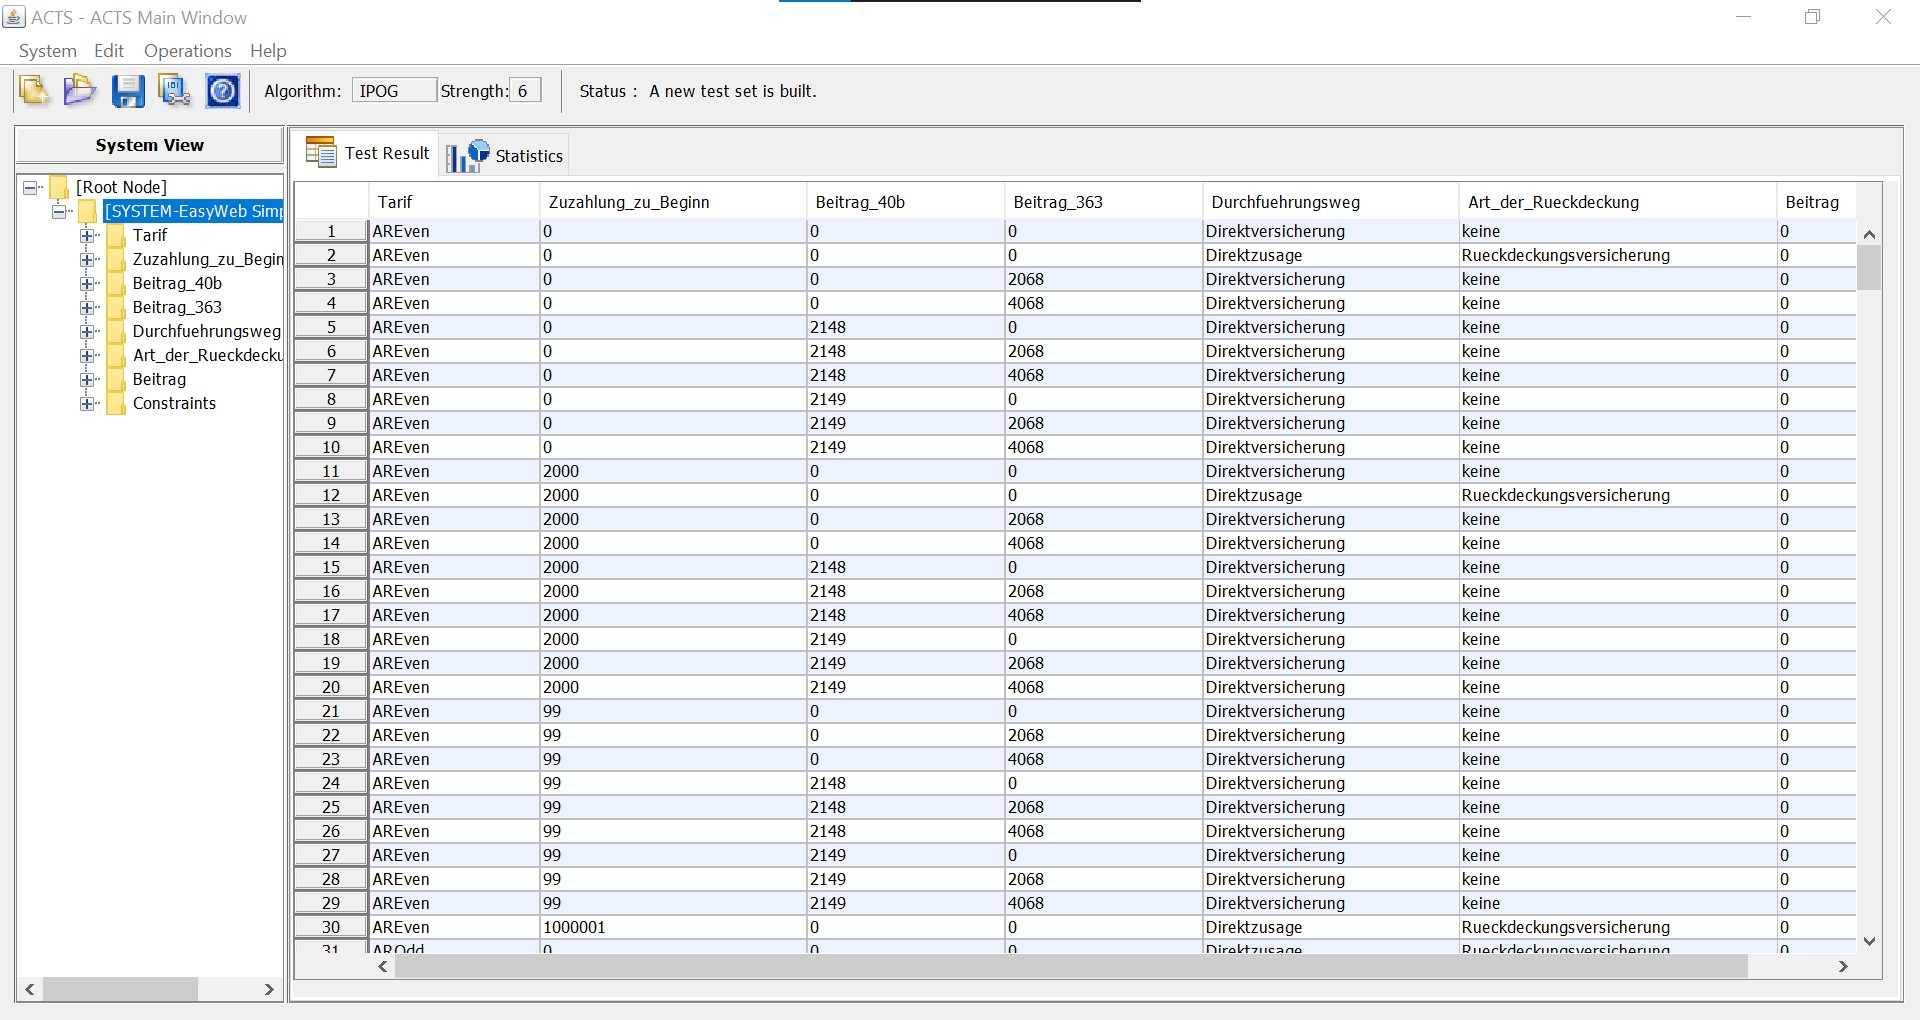
\includegraphics[width=0.8\columnwidth]{images/Screenshot_ACTS.jpg}
\caption{Screenshot der grafischen Benutzeroberfläche von ACTS nach Erstellung eines Covering Arrays. Screenshot erstellt am 15.12.2021.}
\label{fig:acts}
\end{figure}

ACTS ist im Gegensatz zu vielen anderen Tools zur Erstellung von Covering Arrays sehr flexibel in der Art und Weise, wie das zu testende System auszusehen hat und auf welche Art und Weise Testfälle generiert werden sollen: Grundsätzlich kann ACTS Mixed Covering Arrays erstellen: Dies bedeutet, dass die Eingabeparameter eine unterschiedliche Anzahl an verschiedenen Werten annehmen können. Zudem unterstützt ACTS Bedingungen an das Testsystem: Mittels einer speziellen Syntax können bestimmte Parameterbeziehungen durch aussagenlogischen Ausdrücke ausgeschlossen werden. Diese Syntax orientiert sich im Wesentlichen an typischen logischen Operationen \glqq Und\grqq{}, \glqq Oder\grqq{}, \glqq Nicht\grqq{} und arithmetischen Vergleichsoperatoren \glqq $<$\grqq{}, \glqq $>$\grqq{}, \glqq $\leq$\grqq{}, \glqq $\geq$\grqq{} (vgl. dazu \cite{yu2013acts}). Für die Umsetzung dieses Konzepts ist in ACTS ein externes Framework namens Choco \cite{solver} integriert, das für jeden erzeugten Testfall überprüft, ob die zuvor formulierten Bedingungen verletzt werden.

Unter Berücksichtigung dieser Bedingungen, erstellt ACTS Covering Arrays bis zu einer Abdeckung des Interaktionsparameters $t = 6$. Dass ACTS keine Abdeckung höherer Werte für den Interaktionsparameter ermöglicht, liegt darin begründet, dass Kuhn et al. \cite{kuhn2004error} in einer experimentellen Untersuchung aufzeigen konnten, dass fast alle Fehler von Softwaresystemen auf die Interaktion von sechs oder weniger Parameter zurückzuführen sind (vgl. \autoref{sec:combinatorialTesting}). 

ACTS ermöglicht es zudem für verschiedene Gruppen von Eingabeparameter einen unterschiedlichen Wert für den Interaktionsparameter zu fordern und ermöglicht es somit verschiedene Parameterbeziehungen zu priorisieren. In der Literatur wird dies \glqq Mixed Strength Test Generation\grqq{} genannt \cite{yu2013acts, czerwonka2006pairwise}. Wird beispielsweise der Interaktionsparameter $t = 2$ gewählt und es ist jedoch bekannt, dass die Parameter $x_1, x_3, x_4$ und $x_7$ in ihrer Interaktion besonders kritisch zu betrachten sind, so kann für diese Parametermenge bei ACTS eine \glqq Relation\grqq{} \cite{yu2013acts} definiert werden, bei der eine Abdeckung mit $t = 3$ gefordert wird. ACTS besitzt eine interne Logik, die zunächst die verschiedenen Relationen verknüpft und eventuell überflüssige Kombinationen herausfiltert. Erst danach erstellt ACTS eine Übersicht über die zu erstellenden Kombinationen und bildet ein Covering Array \cite{yu2013acts}.

Eine weitere Eigenschaft, welche ACTS abdeckt, ist das explizite Testen auf fehlerhafte Eingaben, sogenanntes \glqq Negative Testing\grqq{} \cite{acts_user_guide}. ACTS bietet die Möglichkeit neben der standardmäßigen Definition der Werte eines Parameters auch explizit Werte zu definieren, die erwartungsgemäß zu Fehler führen sollen. Diese werden dann bei der Erstellung der Menge an Testfällen gesondert berücksichtigt: Konkret bedeutet dies, dass ACTS sicherstellt, dass pro Testfall maximal ein fehlerhafter Wert vorkommen kann. Dies hat das Ziel mögliche Überlagerungen von fehlerhaften Werten zu vermeiden \cite{acts_user_guide}. Zudem erstellt ACTS Testfälle derart, dass jeder fehlerhafte Wert mit jeder $(t-1)$-fachen Kombination von gültigen Werten kombiniert wird \cite{acts_user_guide}.
  
Bei der Erstellung von Covering Arrays haben die Anwender*innen von ACTS die Wahl zwischen verschiedenen Algorithmen: ACTS wurde konzeptionell auf die Nutzung der unterschiedlichen IPOG-Algorithmen ausgerichtet (vgl. \autoref{subsub:ipog}) und besitzt dementsprechend die Auswahlmöglichkeiten des klassischen IPOG-Algorithmus \cite{lei2008ipog}, des IPOG-D-Algorithmus \cite{lei2008ipog} und der beiden IPOG-F-Algorithmen \cite{forbes2008refining} (vgl. \autoref{subsub:ipog}). Darüber hinaus implementierten die Entwickler von ACTS einen zufallsbasierten Algorithmus namens \glqq PaintBall\grqq{}. Zudem existiert bei ACTS die Möglichkeit ein Covering Array im Sinne einer Base Choice-Abdeckung zu erstellen, wie sie in \autoref{subsec:masse} vorgestellt wurde. Beschränkungen bei der Auswahl der Algorithmen ergeben sich jedoch bei der Verwendung der Prinzipien von Mixed Covering Arrays und Constraints: Mixed Covering Arrays und Constraints können nur unter Anwendung des allgemeinen IPOG-Algorithmus und der IPOG-F-Variante erstellt werden. \cite{acts_user_guide}.

Neben der Erzeugung einer Menge von Testfällen zur vollständigen $t$-fachen Abdeckung besteht bei ACTS die Möglichkeit ein bestehendes Covering Array bei Anpassungen der Parameter und deren Werten zu ergänzen ohne dabei eine komplett neue Testfallmenge erstellen zu müssen. Allgemein bietet ACTS für jede Menge an Testfällen zudem die Möglichkeit zu prüfen, ob und inwiefern eine $t$-fache Abdeckung erreicht wird.

\subsubsection{PICT}\label{subsub:pict}
PICT \cite{czerwonka2006pairwise, pict} wurde 2006 erstmalig von Jacek Czerwonka vorgestellt und basiert auf dem AETG-Algorithmus (vgl. \autoref{subsub:aetg}). Das Tool wird über die Kommandozeile angesteuert, nimmt dabei eine Textdatei mit der Spezifikation des Testsystems als Eingabe an und gibt die Menge der erzeugten Testfälle auf der Kommandozeile aus \cite{pict}. Czerwonka \cite{czerwonka2006pairwise} betont, dass sich das entwickelte Tool verstärkt auf die (Rechen-)Effizienz und die Nutzbarkeit im praktischen \glqq Test-Alltag\grqq{} ausrichtet und dementsprechend keine grundlegend neuen Methoden zur Generierung von Covering Arrays beinhaltet. Konkret bedeutet dies: PICT besitzt eine Reihe zusätzlicher Eigenschaften und Funktionalitäten im Vergleich zur allgemeinen Erstellung von Covering Arrays, wie sie beispielsweise im Rahmen vom AETG-Algorithmus durchgeführt werden.

So veränderte Czerwonka den Algorithmus der Erstellung der Covering Arrays des AETG-Ansatzes derart, dass PICT auf Basis eines fest definierten Seeds, also einem vordefinierten Startwert für die Erstellung pseudozufälliger Zahlen, arbeitet und keine zufällige Komponente besitzt (vgl. im Gegensatz dazu \autoref{subsub:aetg}). 

Neben dieser Änderung am Algorithmus selbst fügte Czerwonka verschiedene Optionen ein, welche die Menge der zu erzeugenden Kombinationen, die als Grundlage des Algorithmus dienen, flexibel hält \cite{czerwonka2006pairwise}. Konkret bedeutet dies: Der Interaktionsparameter $t$ kann bei PICT bis zu einem Wert von $t = 6$ beliebig gewählt werden \cite{khalsa2014orchestrated}, zudem unterstützt das Tool das Prinzip der \glqq Mixed Test Strength Generation\grqq{} (vgl. \autoref{subsub:acts}) \cite{czerwonka2006pairwise}. PICT erlaubt es den Anwendenden darüber hinaus eine Hierarchie zu definieren, sodass tiefer positionierte Komponenten nur auf ihrer jeweiligen Hierarchiestufe kombiniert werden können und somit die Anzahl der Testfälle im Gesamten reduziert werden kann \cite{czerwonka2006pairwise}. 

Wie auch ACTS ist PICT in der Lage, Bedingungen des zu testenden Systems zu berücksichtigen: Mittels einer \glqq IF-THEN\grqq{}-Logik kann spezifiziert werden, welche Voraussetzungen die resultierenden Testfälle erfüllen sollen. PICT wandelt diese aussagenlogischen Formeln intern in eine Menge an auszuschließenden Kombinationen um, die dann beim modifizierten AETG-Erzeugungsalgorithmus exkludiert werden \cite{czerwonka2006pairwise}. Eine weitere Ergänzung von PICT ist die Formulierung von \glqq Seeds\grqq{}: Dies sind Testfälle, die in jedem Fall im Covering Array erscheinen müssen. Zudem unterstützt PICT explizit sogenanntes \glqq Negative Testing\grqq{}, also gezieltes Testen auf Fehlverhalten, und die Gewichtung von Werten einzelner Parameter, die bei Don't Cares im Algorithmus berücksichtigt wird.

\begin{comment}

\subsubsection{CTWedge}\label{subsub:ctwedge}

Viele der Tools zur Erstellung von kombinatorischen Testmengen, die in der Vergangenheit vorgestellt wurden, sind Domänen-spezifisch: Dies bedeutet, dass diese meist als Desktop-Anwendungen oder als spezielle Plugins für existierende Software entwickelt wurden und dementsprechend nicht universell einsetzbar sind \cite{gargantini2018migrating}. Um diesem Problem zu begegnen, entwickelten Gargantini und Radavelli \cite{gargantini2018migrating} ein Web-basiertes Tool für Combinatorial Testing \cite{ctwedge}, das die Erstellung von Covering Arrays über einen Server vornimmt und der Zugriff über das Internet erfolgt. Dies wird auch als \glqq Software as a Service\grqq{} bezeichnet \cite{gargantini2018migrating}. Abbildung \ref{fig:ctwedge} zeigt einen Screenshot von CTWedge aus Nutzersicht.

Über eine selbst definierte Syntax, die anhand des domänenspezifischen Modellierungsframeworks Xtext \cite{eysholdt2010xtext} geparst wird, können die Parameter und ihre Werte definiert werden. CTWedge unterstützt genauso wie ACTS die Formulierung von Bedingungen an das Testsystem, die ebenfalls in einer selbst definierten Syntax aufgeschrieben werden müssen. Details zur Syntax können bei Gargantini und Radavelli \cite{gargantini2018migrating} und anhand vordefinierten Beispielen des frei verfügbaren CTWedge-Tools \cite{ctwedge} entnommen werden.

Gargantini und Radavelli verwenden bei der Erzeugung der Testfälle keine eigenen Algorithmen, sondern greifen auf die Schnittstellen anderer Tools zurück: Im Konkreten haben die beiden Autoren die Schnittstelle von ACTS (vgl. \autoref{subsub:acts}) und CASA (vgl. \autoref{subsub:casa}) integriert.

\end{comment}









